\documentclass[a4paper,12pt]{article}
\usepackage[T2A]{fontenc}
\usepackage[utf8]{inputenc}
\usepackage[ukrainian]{babel}
% cmap removed (missing)
\usepackage{t4}

\usepackage{geometry}
% Поле під таблицю в рамці: вирівнюємо по самій рамці
\geometry{
  left=20mm,
  right=5mm,
  top=10mm,
  bottom=10mm
}

\usepackage{anyfontsize}
\usepackage[hidelinks]{hyperref} % щоб працювали посилання без рамок

\usepackage{graphicx}
\usepackage{array,multirow}
\usepackage{booktabs}
\usepackage{caption}

\usepackage{subcaption}

\usepackage{amsmath}
\usepackage{pdflscape}
\usepackage{xcolor}

\usepackage{enumitem}

\usepackage{minted}

\usemintedstyle{friendly} % або monokai / vs / colorful
\setminted{linenos, breaklines, frame=single, fontsize=\small, numbersep=2pt}

\pagestyle{empty} % прибрали стандартну нумерацію

% Підлаштовуємо дані під себе
\renewcommand{\dstuMainTitle}{КУРСОВА РОБОТА}
\renewcommand{\dstuMainSubtitle}{Технічне завдання}
\renewcommand{\dstuCheckName}{Нікольський С.С.}
\renewcommand{\dstuApprName}{Нiкольський С.С.}
\renewcommand{\dstuRecName}{} % Реценз.
\renewcommand{\dstuNkName}{} % Н. контр.

\dstuSetFrameLineWidth{2.33pt}
\dstuSetTopTableStretch{2.06}

\begin{document}

  \dstuPagePlain

  \begin{center}
\includegraphics[width=0.7\textwidth]{../../../TITLES/letterhead.png}\end{center}

  \begin{center}
      \large Національний технічний університет України\\
      «Київський політехнічний інститут імені Ігоря Сікорського»\\[1em]
      Факультет інформатики та обчислювальної техніки\\
      Кафедра обчислювальної техніки
  \end{center}

  \vfill

  \begin{center}
    \textbf{\Large КУРСОВА РОБОТА}\\[1ex]
    \textbf{з дисципліни «Вступ до операційної системи Linux»}
  \end{center}

  \vfill

  \begin{flushleft}
    \hspace*{100mm}% за потреби трохи змінюй (75–85 мм)
    \begin{minipage}{70mm}
      Виконав: Давидчук А.\,М.\\[0.5em]
      Група: ІО-41\\[0.5em]
      Варіант: 4106\\[0.5em]
      Допущений до захисту \rule{25mm}{0.4pt}\\[2ex]
      \rule{70mm}{0.4pt}\\[-0.2ex]\\[0.1em]
      \scriptsize(оцінка, підпис керівника)
    \end{minipage}
  \end{flushleft}

  \vfill

  \begin{center}Київ --- 2025\end{center}

  \newpage

  \dstuPagePlain

  \newgeometry{left=2cm,right=2cm,top=2cm,bottom=2cm}

  \vspace*{0.45\textheight} % вертикальне вирівнювання до центру
  \begin{center}
  \textbf{{\fontsize{50pt}{3pt}\selectfont Опис альбому}}
  \end{center}
  \vspace*{\fill}

  \newpage

  \newgeometry{left=20mm,right=5mm,top=5mm,bottom=5mm}

  \renewcommand{\dstuMainSubtitle}{Опис альбому}
  \renewcommand{\dstuDocCode}{КПІ.ФІОТ.IO4106.001 ОА}
  
  \dstuPageMain
  \dstuTopTable
  \renewcommand{\dstuSheetCount}{1}

  \newpage

  \dstuPagePlain

  \newgeometry{left=2cm,right=2cm,top=2cm,bottom=2cm}

  \vspace*{0.45\textheight} % вертикальне вирівнювання до центру
  \begin{center}
  \textbf{{\fontsize{50pt}{3pt}\selectfont Технічне завдання}}
  \end{center}
  \vspace*{\fill}

  \newpage

  \dstuPageMain

  \newgeometry{
  left=25mm,   % 20мм до рамки + ~5мм від рамки до тексту
  right=10mm,  % 5мм до рамки + ~5мм
  top=15mm,    % 5мм + ~10мм
  bottom=15mm  % 5мм + ~10мм
}

  \renewcommand{\dstuMainSubtitle}{Технічне завдання}
  \renewcommand{\dstuDocCode}{КПІ.ФІОТ.IO4106.002 ТЗ}

  \begin{center}
    \textbf{\Large ЗМІСТ}
  \end{center}

  \hyperref[sec:meta]{\textbf{\textit{1. МЕТА\makebox[13cm][l]{\dotfill}2}}}\\[1em]

  \hyperref[sec:tools]{\textbf{\textit{2. ІНСТРУМЕНТИ ДЛЯ ВИКОНАННЯ КУРСОВОЇ\makebox[3.2cm][l]{\dotfill}2}}}\\[1em]

  \hyperref[sec:stages]{\textbf{\textit{3. ЕТАПИ ВИКОНУВАННЯ РОБОТИ\makebox[6.35cm][l]{\dotfill}2}}}\\[1em]

  \hyperref[sec:docs]{\textbf{\textit{4. ПЕРЕЛІК ТЕКСТОВОЇ ДОКУМЕНТАЦІЇ\makebox[4.9cm][l]{\dotfill}2}}}\\[1em]

  \renewcommand{\dstuSheetCount}{2}

  \newpage

  \dstuPageFull
  \dstuSetSheetNumber{2}

  \begin{center}
    \phantomsection\label{sec:meta}%
    \textbf{\textit{1. МЕТА}}
  \end{center}

  \noindent
  Мета курсової роботи — опанувати роботу з Unix-подібними системами на базі ядра Linux; навчитися створювати репозиторії, редагувати файли, індексувати їх і пушити зміни через Git; збирати програмне забезпечення за допомогою Make, що автоматизує перетворення файлів; писати bash-скрипти для автоматизації задач; а також освоїти інструменти CI/CD на основі Jenkins.

  \vspace{1em}

  \begin{center}
    \phantomsection\label{sec:tools}%
  \textbf{\textit{2. ІНСТРУМЕНТИ ДЛЯ ВИКОНАННЯ КУРСОВОЇ}}
  \end{center}

  \noindent
  Курсову роботу виконуємо з використанням Git як системи контролю версій, Make як утиліти для автоматизації перетворення файлів, bash як стандартної командної оболонки в Unix/Linux, та Jenkins як інструмента безперервної інтеграції.

  \vspace{1em}

  \begin{center}
    \phantomsection\label{sec:stages}%
  \textbf{\textit{3. ЕТАПИ ВИКОНУВАННЯ РОБОТИ}}
  \end{center}

  \noindent
  Під час виконання курсової роботи ми проходимо наступні етапи:

  \begin{enumerate}
    \item Ознайомлення з функціоналом та властивостями Git;
    \item Виконання операцій, вказаних у практичному завданні №1;
    \item Ознайомлення з Make;
    \item Виконання операцій, вказаних у практичному завданні №2;
    \item Ознайомлення з функціоналом bash;
    \item Виконання операцiй, вказаних у практичному завданнi №3;
    \item Ознайомлення з CI/CD інструментами на основі Jenkins;
    \item Виконання операцій, вказаних у практичному завданні №4.
  \end{enumerate}

  \vspace{1em}

  \begin{center}
    \phantomsection\label{sec:docs}%
  \textbf{\textit{4. ПЕРЕЛІК ТЕКСТОВОЇ ДОКУМЕНТАЦІЇ}}
  \end{center}

  \begin{enumerate}
    \item Титульний лист;
    \item Сторінка з написом «Опис альбому»;
    \item Опис альбому;
    \item Сторінка з написом «Технічне завдання»;
    \item Технічне завдання;
    \item Сторінка з написом «Пояснювальна записка»;
    \item Пояснювальна записка.
  \end{enumerate}

  \newpage

  \dstuPagePlain

  \newgeometry{left=2cm,right=2cm,top=2cm,bottom=2cm}

  \vspace*{0.45\textheight} % вертикальне вирівнювання до центру
  \begin{center}
  \textbf{{\fontsize{50pt}{20pt}\selectfont Пояснювальна}}\\[0.5em]
  \textbf{{\fontsize{50pt}{20pt}\selectfont записка}}
  \end{center}
  \vspace*{\fill}

  \newpage

  \dstuPageMain

  \newgeometry{
  left=25mm,   % 20мм до рамки + ~5мм від рамки до тексту
  right=10mm,  % 5мм до рамки + ~5мм
  top=15mm,    % 5мм + ~10мм
  bottom=15mm  % 5мм + ~10мм
}

  \renewcommand{\dstuMainSubtitle}{Пояснювальна записка}
  \renewcommand{\dstuDocCode}{КПІ.ФІОТ.IO4106.003 ПЗ}

  \begin{center}
    \textbf{\Large ЗМІСТ}
  \end{center}

  \hyperref[sec:section1]{\textbf{\textit{1. РОЗДІЛ 1\makebox[12cm][l]{\dotfill}2}}}\\[1em]

  \hyperref[sec:section2]{\textbf{\textit{2. РОЗДІЛ 2\makebox[12cm][l]{\dotfill}9}}}\\[1em]

  \hyperref[sec:section3]{\textbf{\textit{3. РОЗДІЛ 3\makebox[12cm][l]{\dotfill}16}}}\\[1em]

  \hyperref[sec:section4]{\textbf{\textit{4. РОЗДІЛ 4\makebox[12cm][l]{\dotfill}26}}}\\[1em]

  \hyperref[sec:concl]{\textbf{\textit{5. ВИСНОВКИ\makebox[11.5cm][l]{\dotfill}50}}}\\[1em]

  \hyperref[sec:sources]{\textbf{\textit{6. СПИСОК ВИКОРИСТАНИХ ДЖЕРЕЛ\makebox[5.4cm][l]{\dotfill}51}}}

  \dstuSetSheetNumber{1}

  \renewcommand{\dstuSheetCount}{51}

  \newpage

  \dstuPageFull
  \dstuSetSheetNumber{2}

  \newgeometry{
    left=25mm,   % 20мм до рамки + ~5мм від рамки до тексту
    right=10mm,  % 5мм до рамки + ~5мм
    top=15mm,    % 5мм + ~10мм
    bottom=25mm  % 5мм + ~10мм
  }

  \begin{titlepage}

  \begin{center}
    \phantomsection\label{sec:section1}%
    \textbf{\Large 1. РОЗДІЛ 1}
  \end{center}

        % Картинка шапки (по центру, з відступом від верху)
        \begin{center}
\includegraphics[width=0.7\textwidth]{../../../TITLES/letterhead.png}\end{center}

        \begin{center}
            \large Національний технічний університет України\\
            «Київський політехнічний інститут імені Ігоря Сікорського»\\[1em]
            Факультет інформатики та обчислювальної техніки\\
            Кафедра обчислювальної техніки
        \end{center}

        \vfill

        \begin{center}
            \textbf{\LARGE Вступ до операційної системи Linux. Курсова робота}\\[2.5em]
            \textbf{\Large Практична робота №1}\\
            «Введення в GIT»
        \end{center}

        \vfill

        \begin{flushright}
            Виконав: студент 2 курсу ФІОТ, гр. ІО-41\\
            \textit{Давидчук А.~М.}\\[1em]
            Перевірив: \textit{Нікольський С.~С.}
        \end{flushright}

        \vfill

        \begin{center}Київ --- 2025\end{center}

    \end{titlepage}

    % Основний документ:

    \setlength{\parindent}{0em}

    \textbf{\underline{Тема:}} «Введення в GIT».
    
    \vspace{1em}

    \begin{center} \textbf{\Large Практична частина} \end{center}

    Клонуємо репозиторій та переходимо до робочої папки calculator:
    \begin{minted}{bash}
PS C:\Users\artem\OneDrive\Desktop\lab2> git clone https://github.com/SergiiPiatakov/calculator.git
Cloning into 'calculator'...
remote: Enumerating objects: 24, done.
remote: Counting objects: 100% (14/14), done.
remote: Compressing objects: 100% (10/10), done.
remote: Total 24 (delta 5), reused 4 (delta 4), pack-reused 10 (from 1)
Receiving objects: 100% (24/24), done.
Resolving deltas: 100% (5/5), done.
PS C:\Users\artem\OneDrive\Desktop\lab2> cd .\calculator\
    \end{minted}

    Перевірка:
    \begin{minted}{bash}
PS C:\Users\artem\OneDrive\Desktop\lab2\calculator> git log --oneline
4ad40a3 (HEAD -> master, origin/master, origin/HEAD) fix truncation error
cbcb06d formatting: use tabs instead of spaces
669f632 improve calculation accuracy
976f691 add a subtraction operation
f03784b add header guard
9972170 basic implementation
75c0e7c Initial commit
    \end{minted}

    Міняю місцями коміти "\texttt{fix truncation error (4ad40a3)}" та "\texttt{formatting: use tabs}
    
    \texttt{instead of spaces (cbcb06d)}" \, за допомогою \texttt{git rebase -i HEAD~n}:
    \begin{minted}{bash}
PS C:\Users\artem\OneDrive\Desktop\lab2\calculator> git rebase -i HEAD~2
hint: Waiting for your editor to close the file...
    \end{minted}

    В редакторі:
    \begin{minted}{bash}
pick cbcb06d # formatting: use tabs instead of spaces
pick 4ad40a3 # fix truncation error

# Rebase 669f632..4ad40a3 onto 669f632 (2 commands)
#
# Commands:
...
    \end{minted}

    Міняю місцями "\texttt{pick cbcb06d ...}" та "\texttt{pick 4ad40a3 ...}", зберігаю та закриваю вікно і отримую конфлікт:

    \begin{minted}{bash}
Auto-merging calculator.cpp
CONFLICT (content): Merge conflict in calculator.cpp
error: could not apply 4ad40a3... fix truncation error
hint: Resolve all conflicts manually, mark them as resolved with
hint: "git add/rm <conflicted_files>", then run "git rebase --continue".
hint: You can instead skip this commit: run "git rebase --skip".
hint: To abort and get back to the state before "git rebase", run "git rebase --abort".
hint: Disable this message with "git config set advice.mergeConflict false"
Could not apply 4ad40a3... # fix truncation error
    \end{minted}

    Вирішую в редакторі конфлікти у обох файлів у редакторі, додаю їх до \texttt{staging area}, продовжую процес \texttt{rebase} оновлюючи текст повідомлення
    комітів, додавши від себе уточнення \texttt{rearranged} і \texttt{Edited-(rearranged)-by: Davydchuk Artem <marshal.dyachenko@gmail}

    \texttt{.com>}:
    \begin{minted}{bash}
hint: Resolve all conflicts manually, mark them as resolved with
hint: "git add/rm <conflicted_files>", then run "git rebase --continue".
hint: You can instead skip this commit: run "git rebase --skip".
hint: To abort and get back to the state before "git rebase", run "git rebase --abort".
hint: Disable this message with "git config set advice.mergeConflict false"
Could not apply 4ad40a3... # fix truncation error
PS C:\Users\artem\OneDrive\Desktop\lab2\calculator> git add .\calculator.cpp
PS C:\Users\artem\OneDrive\Desktop\lab2\calculator> git rebase --continue 
[detached HEAD 8149318] fix truncation error [rearranged]
 Author: Sergii Piatakov <sergii.piatakov@globallogic.com>
 1 file changed, 1 insertion(+), 1 deletion(-)
Auto-merging calculator.cpp
CONFLICT (content): Merge conflict in calculator.cpp
error: could not apply cbcb06d... formatting: use tabs instead of spaces
hint: Resolve all conflicts manually, mark them as resolved with
hint: "git add/rm <conflicted_files>", then run "git rebase --continue".
hint: You can instead skip this commit: run "git rebase --skip".
hint: To abort and get back to the state before "git rebase", run "git rebase --abort".
hint: Disable this message with "git config set advice.mergeConflict false"
Could not apply cbcb06d... # formatting: use tabs instead of spaces
PS C:\Users\artem\OneDrive\Desktop\lab2\calculator> git add .\calculator.cpp
PS C:\Users\artem\OneDrive\Desktop\lab2\calculator> git rebase --continue 
[detached HEAD 27bda0c] formatting: use tabs instead of spaces [rearranged]
 Author: Sergii Piatakov <sergii.piatakov@globallogic.com>
 2 files changed, 5 insertions(+), 5 deletions(-)
Successfully rebased and updated refs/heads/master.
    \end{minted}

    Тепер дивимось результат:
    \begin{minted}{bash}
PS C:\Users\artem\OneDrive\Desktop\lab2\calculator> git log -3
commit 27bda0c6f5e3f4a474c1a04ea8d37fce1084f1b4 (HEAD -> master)
Author: Sergii Piatakov <sergii.piatakov@globallogic.com>
Date:   Thu Nov 15 15:26:35 2018 +0200

    formatting: use tabs instead of spaces [rearranged]

    Signed-off-by: Sergii Piatakov <sergii.piatakov@globallogic.com>
    Edited-(rearranged)-by: Davydchuk Artem <marshal.dyachenko@gmail.com>

commit 814931806e4b33dd2f09ef9894bed5f710133c2a
Author: Sergii Piatakov <sergii.piatakov@globallogic.com>
Date:   Thu Nov 15 15:28:04 2018 +0200

    fix truncation error [rearranged]

    To convert float to integer the truncation is performed, but the
    rounding is expected.

    Test: Add (4.9, 4.9) should return 10.
    Signed-off-by: Sergii Piatakov <sergii.piatakov@globallogic.com>
    Edited-(rearranged)-by: Davydchuk Artem <marshal.dyachenko@gmail.com>

commit 669f6321a41da2337d975872e9294b8b91139010
Author: Sergii Piatakov <sergii.piatakov@globallogic.com>
Date:   Thu Nov 15 15:21:34 2018 +0200

    improve calculation accuracy

    Allow using float point arguments to avoid truncation.

    Test: Add (4.9, 4.9) should return 10.
    Signed-off-by: Sergii Piatakov <sergii.piatakov@globallogic.com>
    \end{minted}

    Створюємо два патчі в окремій папці \texttt{patches\_step1}, використовуючи "\texttt{git format-patch} ":
    \begin{minted}{bash}
PS C:\Users\artem\OneDrive\Desktop\lab2\calculator> mkdir patches_step1


    Directory: C:\Users\artem\OneDrive\Desktop\lab2\calculator


Mode                 LastWriteTime         Length Name
----                 -------------         ------ ----
d-----        01.10.2025     14:50                patches_step1


PS C:\Users\artem\OneDrive\Desktop\lab2\calculator> git format-patch -2 -o patches_step1
patches_step1/0001-fix-truncation-error-rearranged.patch
patches_step1/0002-formatting-use-tabs-instead-of-spaces-rearranged.patch
    \end{minted}

    Тепер поєднаю "\texttt{improve calculation accuracy}"\,та "\texttt{fix truncation error}"\,в один коміт, використовуючи \texttt{git rebase -i}:

    \begin{minted}{bash}
PS C:\Users\artem\OneDrive\Desktop\lab2\calculator> git rebase -i HEAD~3
hint: Waiting for your editor to close the file...
    \end{minted}

    В редакторі маю таке:
    \begin{minted}{bash}
pick 669f632 # improve calculation accuracy
pick 8149318 # fix truncation error [rearranged]
pick 27bda0c # formatting: use tabs instead of spaces [rearranged]

# Rebase 976f691..27bda0c onto 976f691 (3 commands)
#
# Commands
...
    \end{minted}

    І тут я коміт "\texttt{fix truncation error [rearranged]}" я позначу як \texttt{squash} щоб він злився у попередній
    "\texttt{improve calculation accuracy}":
    \begin{minted}{bash}
pick 669f632 # improve calculation accuracy
squash 7e1603b # fix truncation error [rearranged]
pick fcf6e73 # formatting: use tabs instead of spaces [rearranged]

# Rebase 976f691..fcf6e73 onto 976f691 (3 commands)
#
# Commands:
...
    \end{minted}

    Зберігаю, закриваю та пишу повідомлення до коміту "\texttt{improve calculation accuracy and fix truncation error}"\,зі своєю відміткою авторства
\begin{minted}{bash}
PS C:\Users\artem\OneDrive\Desktop\lab2\calculator> git log --oneline -3
3ec3990 (HEAD -> master) formatting: use tabs instead of spaces [rearranged]
56d74f3 improve calculation accuracy and fix truncation error
976f691 add a subtraction operation
    \end{minted}

    Тепер видаляю верхній коміт \texttt{"formatting: use tabs instead of spaces [rearranged]"} шляхом \texttt{git rebase -i}:

    \begin{minted}{bash}
PS C:\Users\artem\OneDrive\Desktop\lab2\calculator> git rebase -i HEAD~1
    \end{minted}

    І отримую таке в редакторі, де я зміню стан коміта \texttt{pick} на \texttt{drop} щоб видалити його зі історії
    \begin{minted}{bash}
pick 3ec3990 # formatting: use tabs instead of spaces [rearranged]

# Rebase 56d74f3..3ec3990 onto 56d74f3 (1 command)
#
# Commands:
...
    \end{minted}

    Потім зберігаю та закриваю вікно редагування та перевіряю:
    \begin{minted}{bash}
PS C:\Users\artem\OneDrive\Desktop\lab2\calculator> git log --oneline -3 
56d74f3 (HEAD -> master) improve calculation accuracy and fix truncation error
976f691 add a subtraction operation
f03784b add header guar
    \end{minted}

    Тепер перейменовую поточне віддалене сховище на "\texttt{github}" та перевіряю:
    \begin{minted}{bash}
PS C:\Users\artem\OneDrive\Desktop\lab2\calculator> git remote -v 
origin  https://github.com/SergiiPiatakov/calculator.git (fetch)
origin  https://github.com/SergiiPiatakov/calculator.git (push)
PS C:\Users\artem\OneDrive\Desktop\lab2\calculator> git remote rename origin github 
Renaming remote references: 100% (3/3), done.
PS C:\Users\artem\OneDrive\Desktop\lab2\calculator> git remote -v
github  https://github.com/SergiiPiatakov/calculator.git (fetch)
github  https://github.com/SergiiPiatakov/calculator.git (push)
    \end{minted}

    Тепер отримую код з віддаленого сховища \texttt{gitlab} за допомогою \texttt{git fetch} та дослідіть його за допомогою \texttt{git log gitlab/master}:
    \begin{minted}{bash}
PS C:\Users\artem\OneDrive\Desktop\lab2\calculator> git remote add gitlab https://gitlab.com/SergiiPiatakov/calculator.git
PS C:\Users\artem\OneDrive\Desktop\lab2\calculator> git remote -v
github  https://github.com/SergiiPiatakov/calculator.git (fetch)
github  https://github.com/SergiiPiatakov/calculator.git (push)
gitlab  https://gitlab.com/SergiiPiatakov/calculator.git (fetch)
gitlab  https://gitlab.com/SergiiPiatakov/calculator.git (push)
PS C:\Users\artem\OneDrive\Desktop\lab2\calculator> git fetch gitlab
remote: Enumerating objects: 7, done.
remote: Total 7 (delta 0), reused 0 (delta 0), pack-reused 7 (from 1)
Unpacking objects: 100% (7/7), 903 bytes | 31.00 KiB/s, done.
From https://gitlab.com/SergiiPiatakov/calculator
 * [new branch]      master     -> gitlab/master
PS C:\Users\artem\OneDrive\Desktop\lab2\calculator> git log --oneline gitlab/master
d61d32d (gitlab/master, gitlab/HEAD) mark member-function as `static`
e0ea21b add a multiplication operation
9972170 basic implementation
75c0e7c Initial commit
    \end{minted}

    Потім додаю коміт: "\texttt{add a multiplication operation (e0ea21b)}" використовуючи \texttt{git}

    \texttt{cherry-pick}, вирішую конфлікти у редакторі та завершую операцію \texttt{cherry-pick}:

    \begin{minted}{bash}
PS C:\Users\artem\OneDrive\Desktop\lab2\calculator> git cherry-pick e0ea21b
Auto-merging calculator.cpp
Auto-merging calculator.h
CONFLICT (content): Merge conflict in calculator.h
error: could not apply e0ea21b... add a multiplication operation
hint: After resolving the conflicts, mark them with
hint: "git add/rm <pathspec>", then run
hint: "git cherry-pick --continue".
hint: You can instead skip this commit with "git cherry-pick --skip".
hint: To abort and get back to the state before "git cherry-pick",
hint: run "git cherry-pick --abort".
hint: Disable this message with "git config set advice.mergeConflict false"
PS C:\Users\artem\OneDrive\Desktop\lab2\calculator> git add .\calculator.h  
PS C:\Users\artem\OneDrive\Desktop\lab2\calculator> git cherry-pick --continue 
[master 1fa8ece] add a multiplication operation
 Author: Sergii Piatakov <sergii.piatakov@globallogic.com>
 Date: Thu Nov 15 15:43:25 2018 +0200
 2 files changed, 6 insertions(+)
    \end{minted}

    І перевіряємо результат:

    \begin{minted}{bash}
PS C:\Users\artem\OneDrive\Desktop\lab2\calculator> git log --oneline
1fa8ece (HEAD -> master) add a multiplication operation
56d74f3 improve calculation accuracy and fix truncation error
976f691 add a subtraction operation
f03784b add header guard
9972170 basic implementation
75c0e7c Initial commit
    \end{minted}

    Тепер створю власне виправлення на 5-15 рядків коду (додавши ще функцію ділення) та внесу зміни:
    \begin{minted}{bash}
PS C:\Users\artem\OneDrive\Desktop\lab2\calculator> git add .\calculator.cpp
PS C:\Users\artem\OneDrive\Desktop\lab2\calculator> git add .\calculator.h  
PS C:\Users\artem\OneDrive\Desktop\lab2\calculator> git commit -m "new function: Div" 
[master 2bcb78d] new function: Div
 2 files changed, 6 insertions(+)
    \end{minted}

    Та надсилаю результат у власний репозиторій:

    \begin{minted}{bash}
PS C:\Users\artem\OneDrive\Desktop\lab2\calculator> git remote add my_lab2_repo https://github.com/davidchyk/coursework-calculator-lab2.git
PS C:\Users\artem\OneDrive\Desktop\lab2\calculator> git push -u my_lab2_repo master
Enumerating objects: 25, done.
Counting objects: 100% (25/25), done.
Delta compression using up to 16 threads
Compressing objects: 100% (22/22), done.
Writing objects: 100% (25/25), 2.76 KiB | 943.00 KiB/s, done.
Total 25 (delta 6), reused 12 (delta 2), pack-reused 0 (from 0)
remote: Resolving deltas: 100% (6/6), done.
To https://github.com/davidchyk/coursework-calculator-lab2.git
 * [new branch]      master -> master
branch 'master' set up to track 'my_lab2_repo/master'.
    \end{minted}

    \textbf{\underline{Висновок:}} У ході виконання лабораторної роботи було опановано основні інструменти Git: 
зміну порядку комітів за допомогою \texttt{git rebase -i}, їх об’єднання (\texttt{squash}), 
видалення (\texttt{drop}), а також використання команди \texttt{cherry-pick} для 
перенесення змін з віддаленого репозиторію. Створено та підписано патчі за допомогою 
\texttt{git format-patch}.

\setlength{\parindent}{1.5em}

У результаті виконано виправлення похибки округлення, об’єднано коміти 
\texttt{"improve"}
\texttt{"calculation accuracy}"\,та \texttt{"fix truncation error"}, видалено службовий 
коміт форматування, додано операцію множення з версії GitLab та реалізовано власне 
виправлення --- функцію ділення з перевіркою на нуль і округленням результату.  

Таким чином, мету роботи досягнуто: набуті практичні навички роботи з історією 
комітів у Git, вирішення конфліктів, створення та застосування патчів, а також 
розширення функціоналу класу \texttt{Calculator}.

\newpage

  \begin{titlepage}

    \begin{center}
    \phantomsection\label{sec:section2}%
    \textbf{\Large 2. РОЗДІЛ 2}
    \end{center}

        % Картинка шапки (по центру, з відступом від верху)
        \begin{center}
\includegraphics[width=0.7\textwidth]{../../../TITLES/letterhead.png}\end{center}

        \begin{center}
            \large Національний технічний університет України\\
            «Київський політехнічний інститут імені Ігоря Сікорського»\\[1em]
            Факультет інформатики та обчислювальної техніки\\
            Кафедра обчислювальної техніки
        \end{center}

        \vfill

        \begin{center}
            \textbf{\LARGE Вступ до операційної системи Linux. Курсова робота}\\[2.5em]
            \textbf{\Large Практична робота №2}\\[1em]
            «Розроблення Makefile та CMake файлiв»
        \end{center}

        \vfill

        \begin{flushright}
            Виконав: студент 2 курсу ФІОТ, гр. ІО-41\\
            \textit{Давидчук А.~М.}\\[1em]
            Перевірив: \textit{Нікольський С.~С.}
        \end{flushright}

        \vfill

        \begin{center}Київ --- 2025\end{center}

    \end{titlepage}

    % Основний документ:

    \setlength{\parindent}{0em}

    \textbf{\underline{Тема:}} «Розроблення Makefile та CMake файлiв».
    
    \vspace{1em}

    \begin{center} \textbf{\Large Практична частина} \end{center}

    Використовуватиму минулий репозиторiй iз лабораторної роботи №2 (практична робота №1):
    \begin{minted}{bash}
PS C:\Users\artem\OneDrive\Desktop\coursework-calculator-lab2-3> git log --oneline
2bcb78d (HEAD -> master, origin/master, origin/HEAD) new function: Div
1fa8ece add a multiplication operation
56d74f3 improve calculation accuracy and fix truncation error
976f691 add a subtraction operation
f03784b add header guard
9972170 basic implementation
75c0e7c Initial commit
    \end{minted}

    Тут створю основний файл програми main.cpp:

    \begin{minted}{cpp}
#include <iostream>
#include "calculator.h"

int main() {
    Calculator c;
    std::cout << "2 + 3 = " << c.Add(2, 3) << "\n";
    std::cout << "5 - 1 = " << c.Sub(5, 1) << "\n";
    std::cout << "4 * 2 = " << c.Mul(4, 2) << "\n";
    std::cout << "9 / 3 = " << c.Div(9, 3) << "\n";

    return 0;
}
    \end{minted}

    А також файл CMakeLists.txt:

    \begin{minted}{text}
cmake_minimum_required(VERSION 3.10)
project(calculator_project LANGUAGES CXX)

set(CMAKE_CXX_STANDARD 11)
set(CMAKE_CXX_STANDARD_REQUIRED ON)

# Output directories
set(CMAKE_RUNTIME_OUTPUT_DIRECTORY ${CMAKE_BINARY_DIR}/bin)
set(CMAKE_ARCHIVE_OUTPUT_DIRECTORY ${CMAKE_BINARY_DIR}/lib)

add_library(calculator STATIC
    calculator.cpp
)
target_include_directories(calculator PUBLIC include)

add_executable(calc_app
    main.cpp
)
target_link_libraries(calc_app PRIVATE calculator)
    \end{minted}

    I разом iз ним файл Makefile:

    \begin{minted}{text}
# Makefile для MSVC

CC=cl
AR=lib
CFLAGS=/nologo /W4 /O2 /EHsc /I.
LDFLAGS=/nologo

OUTDIR=build
BINDIR=$(OUTDIR)\bin
LIBDIR=$(OUTDIR)\lib
OBJDIR=$(OUTDIR)\obj

APP=$(BINDIR)\calc_app.exe
LIB=$(LIBDIR)\calculator.lib

.PHONY: all clean dirs

all: dirs $(APP)

dirs:
	if not exist $(OUTDIR) mkdir $(OUTDIR)
	if not exist $(BINDIR) mkdir $(BINDIR)
	if not exist $(LIBDIR) mkdir $(LIBDIR)
	if not exist $(OBJDIR) mkdir $(OBJDIR)

$(OBJDIR)\calculator.obj: calculator.cpp calculator.h
	$(CC) $(CFLAGS) /c calculator.cpp /Fo$(OBJDIR)\calculator.obj

$(LIB): $(OBJDIR)\calculator.obj | dirs
	$(AR) /nologo /OUT:$(LIB) $(OBJDIR)\calculator.obj

$(OBJDIR)\main.obj: main.cpp calculator.h
	$(CC) $(CFLAGS) /c main.cpp /Fo$(OBJDIR)\main.obj

$(APP): $(OBJDIR)\main.obj $(LIB) | dirs
	$(CC) $(LDFLAGS) $(OBJDIR)\main.obj $(LIB) /Fe$(APP)

clean:
	- del /Q /F $(OBJDIR)\*.obj 2>nul
	- del /Q /F $(LIB) 2>nul
	- del /Q /F $(APP) 2>nul
	- rmdir /S /Q $(OUTDIR) 2>nul
    \end{minted}

    Звiдси маю таку структуру робочої областi:

    \begin{minted}{text}
PS C:\Users\artem\OneDrive\Desktop\coursework-calculator-lab2-3> tree /f
Folder PATH listing
Volume serial number is 7667-D297
C:.
    calculator.cpp
    calculator.h
    CMakeLists.txt
    main.cpp
    Makefile

No subfolders exist
    \end{minted}

    Збiрка проєкту виконується на основi CMakeLists.txt з використанням системи збирання
Ninja:

    \begin{minted}{text}
PS C:\Users\artem\OneDrive\Desktop\coursework-calculator-lab2-3> cmake -S . -B build-ninja -G Ninja -DCMAKE_BUILD_TYPE=Release
-- The CXX compiler identification is GNU 13.2.0
-- Detecting CXX compiler ABI info
-- Detecting CXX compiler ABI info - done
-- Check for working CXX compiler: C:/Strawberry/c/bin/c++.exe - skipped
-- Detecting CXX compile features
-- Detecting CXX compile features - done
-- Configuring done (1.0s)
-- Generating done (0.0s)
-- Build files have been written to: C:/Users/artem/OneDrive/Desktop/coursework-calculator-lab2-3/build-ninja
PS C:\Users\artem\OneDrive\Desktop\coursework-calculator-lab2-3> ninja -C build-ninja
ninja: Entering directory `build-ninja`
[4/4] Linking CXX executable bin\calc_app.exe
    \end{minted}

    I запускаю отриману програму:

    \begin{minted}{text}
PS C:\Users\artem\OneDrive\Desktop\coursework-calculator-lab2-3> build-ninja\bin\calc_app.exe
2 + 3 = 5
5 - 1 = 4
4 * 2 = 8
9 / 3 = 3
    \end{minted}

    Що свiдчить про успiшнiсть збiрки. Робоча область тепер має таку структуру:

    \begin{minted}{text}
PS C:\Users\artem\OneDrive\Desktop\coursework-calculator-lab2-3> tree /f /a
Folder PATH listing
Volume serial number is 7667-D297
C:.
|    calculator.cpp
|    calculator.h
|    CMakeLists.txt
|    main.cpp
|    Makefile
|
\---build-ninja
    |    .ninja_deps
    |    .ninja_log
    |    build.ninja
    |    CMakeCache.txt
    |    cmake_install.cmake
    |
    +---bin
    |       calc_app.exe
    |
    +---CMakeFiles
    |   |   cmake.check_cache
    |   |   CMakeConfigureLog.yaml
    |   |   rules.ninja
    |   |   TargetDirectories.txt
    |   |
        +---3.29.2
    |   |   |   CMakeCXXCompiler.cmake
    |   |   |   CMakeDetermineCompilerABI_CXX.bin
    |   |   |   CMakeRCCompiler.cmake
    |   |   |   CMakeSystem.cmake
    |   |   |
    |   |   \---CompilerIdCXX
    |   |       |   a.exe
    |   |       |   CMakeCXXCompilerId.cpp
    |   |       |
    |   |       \---tmp
    |   +---calculator.dir
    |   |       calculator.cpp.obj
    |   |
    |   +---calc_app.dir
    |   |       main.cpp.obj
    |   |
    |   +---CMakeScratch
    |   \---pkgRedirects
    \---lib
        libcalculator.a
    \end{minted}

    Також можемо очистити всi артефакти командою \texttt{ninja -C build-ninja -t clean}:

    \begin{minted}{text}
PS C:\Users\artem\OneDrive\Desktop\coursework-calculator-lab2-3> ninja -C build-ninja -t clean
Cleaning... 4 files.
PS C:\Users\artem\OneDrive\Desktop\coursework-calculator-lab2-3> tree /F /a
Folder PATH listing
Volume serial number is 7667-D297

C:.
|   calculator.cpp
|   calculator.h
|   CMakeLists.txt
|   main.cpp
|   Makefile
|
\---build-ninja
|   |   .ninja_deps
|   |   .ninja_log
|   |   build.ninja
|   |   CMakeCache.txt
|   |   cmake_install.cmake
|   |
|   +---bin
|   +---CMakeFiles
|   |   |   cmake.check_cache
|   |   |   CMakeConfigureLog.yaml
|   |   |   rules.ninja
|   |   |   TargetDirectories.txt
|   |   |
|   |   +---3.29.2
|   |       |   CMakeCXXCompiler.cmake
|   |       |   CMakeDetermineCompilerABI_CXX.bin
|   |       |   CMakeRCCompiler.cmake
|   |       |   CMakeSystem.cmake
|   |       |
|   |       \---CompilerIdCXX
|   |           |   a.exe
|   |           |   CMakeCXXCompilerId.cpp
|   |           |
|   |           \---tmp
|   |
|   +---calculator.dir
|   +---calc_app.dir
|   +---CMakeScratch
|   \---pkgRedirects
\---lib
    \end{minted}

    Тепер збережемо всi новi змiни (файли вихiдного коду, \texttt{Makefile} та \texttt{CMakeLists.txt}) та
вiдправимо їх на вiддалений репозиторiй:

    \begin{minted}{text}
PS C:\Users\artem\OneDrive\Desktop\coursework-calculator-lab2-3> git status
On branch master
Your branch is up to date with 'origin/master'.

Untracked files:
  (use "git add <file>..." to include in what will be committed)
        CMakeLists.txt
        Makefile
        build-ninja/
        main.cpp

nothing added to commit but untracked files present (use "git add" to track)
PS C:\Users\artem\OneDrive\Desktop\coursework-calculator-lab2-3> git add .\CMakeLists.txt .\Makefile .\main.cpp
warning: in the working copy of 'CMakeLists.txt', LF will be replaced by CRLF the next time Git touches it
warning: in the working copy of 'Makefile', LF will be replaced by CRLF the next time Git touches it
PS C:\Users\artem\OneDrive\Desktop\coursework-calculator-lab2-3> git status
On branch master
Your branch is up to date with 'origin/master'.

Changes to be committed:
  (use "git restore --staged <file>..." to unstage)
        new file:   CMakeLists.txt
        new file:   Makefile
        new file:   main.cpp

Untracked files:
  (use "git add <file>..." to include in what will be committed)
        build-ninja/

PS C:\Users\artem\OneDrive\Desktop\coursework-calculator-lab2-3> git commit -m "new files: main.cpp, CMakeLists.txt and Makefile; Lab#3 (Task #2)"
[master 0ea73d8] new files: main.cpp, CMakeLists.txt and Makefile; Lab#3 (Task #2)
 3 files changed, 73 insertions(+)
 create mode 100644 CMakeLists.txt
 create mode 100644 Makefile
 create mode 100644 main.cpp
PS C:\Users\artem\OneDrive\Desktop\coursework-calculator-lab2-3> git push
Enumerating objects: 6, done.
Counting objects: 100% (6/6), done.
Delta compression using up to 16 threads
Compressing objects: 100% (5/5), done.
Writing objects: 100% (6/6), 1.24 KiB | 1.24 MiB/s, done.
Total 6 (delta 0), reused 0 (delta 0), pack-reused 0 (from 0)
To https://github.com/davidchyk/coursework-calculator-lab2-3.git
   2bcb78d..0ea73d8  master -> master
    \end{minted}

    \textbf{Висновок:} У цій лабораторній роботі було створено мінімальний проєкт,
розроблено \texttt{Makefile} (із \texttt{clean}) та \texttt{CMakeLists.txt}. На основі
\texttt{CMakeLists.txt} згенеровано сценарії збірки для \texttt{Ninja}
(\texttt{build.ninja}, \texttt{rules.ninja}) командою:
\texttt{cmake -S . -B build-ninja -G Ninja}

\texttt{-DCMAKE\_BUILD\_TYPE=Release}. Зібрано одну статичну бібліотеку (\texttt{calculator.lib}

/\texttt{libcalculator.a}) та
виконуваний файл \texttt{calc\_app.exe}; запуск підтвердив коректну роботу.

\newpage

  \begin{titlepage}

  \begin{center}
    \phantomsection\label{sec:section3}%
    \textbf{\Large 3. РОЗДІЛ 3}
  \end{center}

        % Картинка шапки (по центру, з відступом від верху)
        \begin{center}
\includegraphics[width=0.7\textwidth]{../../../TITLES/letterhead.png}\end{center}

        \begin{center}
            \large Національний технічний університет України\\
            «Київський політехнічний інститут імені Ігоря Сікорського»\\[1em]
            Факультет інформатики та обчислювальної техніки\\
            Кафедра обчислювальної техніки
        \end{center}

        \vfill

        \begin{center}
            \textbf{\LARGE Вступ до операційної системи Linux. Курсова робота}\\[1.5em]
            \textbf{\Large Практична робота №3}\\[1em]
            «Створення bash-скрипта за варіантом»
        \end{center}

        \vfill

        \begin{flushright}
            Виконав: студент 2 курсу ФІОТ, гр. ІО-41\\
            \textit{Давидчук А.~М.}\\[1em]
            Перевірив: \textit{Нікольський С.~С.}
        \end{flushright}

        \vfill

        \begin{center}Київ --- 2025\end{center}

    \end{titlepage}

    % Основний документ:

    \setlength{\parindent}{0em}

    \textbf{\underline{Тема:}} «Створення bash-скрипта за варіантом».
    
    \vspace{1em}

    \begin{center} \textbf{\Large Практична частина} \end{center}

    Опис всіх скриптів:

    \begin{enumerate}[label=\arabic*., start=0, itemsep=0.6em, leftmargin=*, align=left]

\item Скрипт приймає два числові параметри.
Якщо 1-й параметр більше 2-го -- вивести відповідне повідомлення, а
також список псевдонімів (alias) вашої системи.
Якщо 1-й параметр не більше 2-го -- вивести відповідне
повідомлення, а також розмір файлу скрипта (назва скрипта має
визначатися всередині самого скрипта).

\item В порядку зростання вивести на екран вагу та назву 3-х найбільш
“важких” директорій (просто файли пропускаються), що знаходиться
в директорії знаходження скрипта.

\item Пройтися по вмісту цільової директорії.
Для кожної директорії -- вивести повідомлення, що \emph{current\_dirname}
є директорією.
Якщо знайдений файл -- створити директорію \emph{current\_filename}\_dir,
і перемістити файл в неї. Вивести повідомлення, що
\emph{current\_filename} переміщений.

\item Згенерувати та записати до файлу 5 випадкових додатних чисел.
Вивести їх на екран. Видалити з файлу всі числа крім найменшого.
Результат вивести на екран.

\item Комбінація з двох маленьких скриптів.
Перший двічі рекурсивно проходить по вмісту цільової директорії,
спочатку видаляючи порожні файли, а потім порожні директорії.
Другий повинен запускати перший скрипт в новому вікні терміналу.
Створене вікно терміналу не повинно автоматично закриватися після
виконання скрипта.

\item Перенаправити результат виконання утиліти “top” в файл.
Обрізати кінець файлу, залишивши в ньому тільки перші n рядків. $n$
передається у якості параметру скрипта. Якщо параметр не було
задано, використовується значення 5.

\end{enumerate}

    Структура робочої директорії:

    \begin{minted}{text}
davydchuk@artem-laptop:~/Desktop/lab$ tree --charset=ascii
.
|-- 0file
|-- 1file
|   `-- file
|-- emptyfile.txt
|-- taskNo0.sh
|-- taskNo1.sh
|-- taskNo2.sh
|-- taskNo3.sh
|-- taskNo4_main.sh
|-- taskNo4_terminal.sh
`-- taskNo5.sh

3 directories, 9 files
    \end{minted}

    \newpage

    Код 1 скрипта (\texttt{taskNo0.sh}):

    \begin{minted}{bash}
#!/usr/bin/env bash
# taskNo0.sh - якщо $1 > $2 -> показати alias-и; інакше -> показати розмір цього скрипта
set -euo pipefail

[[ $# -eq 2 ]] || { echo "Використання: $0 <int1> <int2>"; exit 1; }
re='^-?[0-9]+$'
[[ $1 =~ $re && $2 =~ $re ]] || { echo "Параметри мають бути цілими числами"; exit 1; }

a=$1 b=$2
me=${BASH_SOURCE[0]}

if (( a > b )); then
  echo "Перший параметр ($a) > другого ($b). Alias-и:"
  alias 2>/dev/null || echo "(alias-и не визначені)"
else
  echo "Перший параметр ($a) <= другого ($b)."
  size=$(stat -c %s -- "$me" 2>/dev/null || wc -c < "$me")
  echo "Файл скрипта: $me"
  echo "Розмір скрипта: $size байт(и)"
fi
    \end{minted}

    Перевірка:
    \begin{minted}{bash}
davydchuk@artem-laptop:~/Desktop/lab$ ./taskNo0.sh
Використання: ./taskNo0.sh <int1> <int2>
davydchuk@artem-laptop:~/Desktop/lab$ ./taskNo0.sh 1 2
Перший параметр (1) <= другого (2).
Файл скрипта: ./taskNo0.sh
Розмір скрипта: 816 байт(и)
davydchuk@artem-laptop:~/Desktop/lab$ ./taskNo0.sh 2 1
Перший параметр (2) > другого (1). Alias-и:
    \end{minted}

    Код 2 скрипта (\texttt{taskNo1.sh}):

    \begin{minted}{bash}
#!/usr/bin/env bash
# taskNo1.sh - 3 найважчі піддиректорії біля скрипта; вивід за зростанням
set -euo pipefail

SCRIPT_DIR="$(cd -- "$(dirname -- "${BASH_SOURCE[0]}")" && pwd -P)"

# Якщо піддиректорій немає - повідомляємо і виходимо
if ! find "$SCRIPT_DIR" -mindepth 1 -maxdepth 1 -type d -print -quit | grep -q .; then
  echo "Поруч зі скриптом немає жодної піддиректорії"
  exit 0
fi

# Ланцюжок: перелік піддиректорій → їх розмір (у байтах) → топ-3 найбільші → відсортовано за зростанням
find "$SCRIPT_DIR" -mindepth 1 -maxdepth 1 -type d -print0 \
| xargs -0 -r du -sB1 \
| sort -n \
| tail -n 3 \
| sort -n \
| while read -r bytes path; do
    if command -v numfmt >/dev/null 2>&1; then
      human=$(numfmt --to=iec --suffix=B --format="%.1f" "$bytes")
    else
      human="${bytes}B"
    fi
    printf "%s\t%s\n" "$human" "${path##*/}"
  done
    \end{minted}

    Перевірка:
    \begin{minted}{bash}
davydchuk@artem-laptop:~/Desktop/lab$ ./taskNo1.sh
4,0KB 0file
8,0KB 1file
    \end{minted}

    Код 3 скрипта (\texttt{taskNo2.sh}):

    \begin{minted}{bash}
#!/usr/bin/env bash
# taskNo2.sh - пройтись по вмісту каталогу
set -euo pipefail

TARGET_DIR="${1:-.}"
[[ -d "$TARGET_DIR" ]] || { echo "Помилка: це не директорія: $TARGET_DIR" >&2; exit 1; }

# Перебір лише першого рівня (включно з прихованими). Отримаємо БАЗОВІ імена через %P.
while IFS= read -r -d '' name; do
  path="$TARGET_DIR/$name"

  if [[ -d "$path" ]]; then
    printf "%s є директорією\n" "$name"

  elif [[ -f "$path" || ( -L "$path" && ! -d "$path" ) ]]; then
    dest="$TARGET_DIR/${name}_dir"
    mkdir -p -- "$dest"

    target="$dest/$name"
    if [[ -e "$target" ]]; then
      i=1
      while [[ -e "$dest/${name}.dup${i}" ]]; do ((i++)); done
      target="$dest/${name}.dup${i}"
    fi

    mv -- "$path" "$target"
    printf "%s переміщений\n" "$name"

  else
    printf "%s пропущено (не файл і не директорія)\n" "$name"
  fi
done < <(find "$TARGET_DIR" -mindepth 1 -maxdepth 1 -printf '%P\0' | sort -z)
    \end{minted}

    Перевірка:
    \begin{minted}{bash}
davydchuk@artem-laptop:~/Desktop/lab$ ./taskNo2.sh
0file є директорією
1file є директорією
emptyfile.txt переміщений
taskNo0.sh переміщений
taskNo1.sh переміщений
taskNo2.sh переміщений
taskNo3.sh переміщений
taskNo4_main.sh переміщений
taskNo4_terminal.sh переміщений
taskNo5.sh переміщений
davydchuk@artem-laptop:~/Desktop/lab$ tree --charset=ascii
.
|-- 0file
|-- 1file
|   `-- file
|-- emptyfile.txt_dir
|   `-- emptyfile.txt
|-- taskNo0.sh_dir
|   `-- taskNo0.sh
|-- taskNo1.sh_dir
|   `-- taskNo1.sh
|-- taskNo2.sh_dir
|   `-- taskNo2.sh
|-- taskNo3.sh_dir
|   `-- taskNo3.sh
|-- taskNo4_main.sh_dir
|   `-- taskNo4_main.sh
|-- taskNo4_terminal.sh_dir
|   `-- taskNo4_terminal.sh
`-- taskNo5.sh_dir
    `-- taskNo5.sh

11 directories, 9 files
    \end{minted}

    І для подальшого демонстрування виконання скриптів, я переміщу всі файли назад (тобто дерево файлів повернеться у стан до виконання скрипту \texttt{taskNo2.sh}):

    \begin{minted}{bash}
davydchuk@artem-laptop:~/Desktop/lab$ tree --charset=ascii
.
|-- 0file
|-- 1file
|   `-- file
|-- emptyfile.txt
|-- taskNo0.sh
|-- taskNo1.sh
|-- taskNo2.sh
|-- taskNo3.sh
|-- taskNo4_main.sh
|-- taskNo4_terminal.sh
`-- taskNo5.sh

3 directories, 9 files
    \end{minted}

    Код 4 скрипта (\texttt{taskNo3.sh}):

    \begin{minted}{bash}
#!/usr/bin/env bash
# taskNo3.sh - згенерувати 5 додатних чисел, записати у файл, лишити мінімальне
set -euo pipefail

out="${1:-numbers.txt}"

# Згенерувати 5 чисел (1..1e6), показати й записати у файл
nums=$(for _ in {1..5}; do echo $(( (RANDOM<<15 | RANDOM) % 1000000 + 1 )); done)
printf "%s\n" $nums | tee "$out" >/dev/null

echo "Згенеровані числа:"
printf "%s " $nums; echo

# Знайти мінімум і перезаписати файл лише ним
min=$(printf "%s\n" $nums | sort -n | head -n1)
printf "%s\n" "$min" > "$out"

echo "Мінімальне число (залишено у файлі $out): $min"
echo "Вміст файлу після очистки:"
cat "$out"
    \end{minted}

    Перевірка:
    \begin{minted}{bash}
davydchuk@artem-laptop:~/Desktop/lab$ ./taskNo3.sh
Згенеровані числа:
999923 649956 433307 786355 839671 
Мінімальне число (залишено у файлі numbers.txt): 433307
Вміст файлу після очистки:
433307
davydchuk@artem-laptop:~/Desktop/lab$ tree --charset=ascii
.
|-- 0file
|-- 1file
|   `-- file
|-- emptyfile.txt
|-- numbers.txt
|-- taskNo0.sh
|-- taskNo1.sh
|-- taskNo2.sh
|-- taskNo3.sh
|-- taskNo4_main.sh
|-- taskNo4_terminal.sh
`-- taskNo5.sh

3 directories, 10 files
davydchuk@artem-laptop:~/Desktop/lab$ cat numbers.txt
433307
    \end{minted}

    Код 5 скрипта (обгортки) (\texttt{taskNo4\_terminal.sh}):

    \begin{minted}{bash}
#!/usr/bin/env bash
# taskNo4_terminal.sh - відкрити НОВЕ вікно терміналу, запустити taskNo4_main.sh і залишити вікно відкритим
set -euo pipefail

SELF_DIR="$(cd -- "$(dirname -- "${BASH_SOURCE[0]}")" && pwd -P)"
MAIN="$SELF_DIR/taskNo4_main.sh"

# 1) Визначаємо ціль: якщо не задано - беремо поточну директорію В МОМЕНТ ЗАПУСКУ і робимо її абсолютною
RAW_TARGET="${1:-$(pwd -P)}"
# realpath з фолбеком
if ! TARGET="$(realpath -- "$RAW_TARGET" 2>/dev/null)"; then
  TARGET="$RAW_TARGET"
fi

[[ -x "$MAIN" ]] || { echo "Помилка: зроби виконуваним $MAIN (chmod +x taskNo4_main.sh)" >&2; exit 1; }

# Якщо немає GUI - виконаємо в поточному терміналі з паузою
if [[ -z "${DISPLAY:-}" && -z "${WAYLAND_DISPLAY:-}" ]]; then
  bash --noprofile --norc "$MAIN" "$TARGET" || true
  read -r -p "Натисни Enter, щоб завершити..." _
  exit 0
fi

# Команда для нового вікна: просто викликаємо main з АБСОЛЮТНОЮ ціллю, потім пауза
inner=$(printf "%q " "$MAIN" "$TARGET")
inner+=$'; echo; echo "Завершено"; read -n1 -s -r -p "Натисни будь-яку клавішу, щоб закрити..."'

if command -v gnome-terminal >/dev/null 2>&1; then
  gnome-terminal -- bash --noprofile --norc -c "$inner"
elif command -v konsole >/dev/null 2>&1; then
  konsole --noclose -e bash --noprofile --norc -c "$inner"
elif command -v xfce4-terminal >/dev/null 2>&1; then
  xfce4-terminal --hold -e bash --noprofile --norc -c "$inner"
elif command -v kitty >/dev/null 2>&1; then
  kitty bash --noprofile --norc -c "$inner"
elif command -v alacritty >/dev/null 2>&1; then
  alacritty -e bash --noprofile --norc -c "$inner"
elif command -v xterm >/dev/null 2>&1; then
  xterm -hold -e bash --noprofile --norc -c "$inner"
else
  echo "Не знайдено відомого GUI-термінала. Встанови, напр.: sudo pacman -S xterm" >&2
  exit 1
fi
    \end{minted}

    Код 5 скрипта (основна логіка) (\texttt{taskNo4\_main.sh}):

    \begin{minted}{bash}
#!/usr/bin/env bash
# taskNo4_main.sh - спершу видаляє порожні файли, потім порожні директорії (рекурсивно)
set -euo pipefail

DIR="${1:-.}"
[[ -d $DIR ]] || { echo "Помилка: '$DIR' не існує або не є директорією" >&2; exit 1; }

printf "Цільова директорія: %s\n" "$DIR"
printf "Крок 1: Знаходимо порожні файли\n"
find -P "$DIR" -type f -empty -print -delete || true

printf "\nКрок 2: Знаходимо порожні директорії\n"
find -P "$DIR" -depth -type d -empty -print -delete || true

echo -e "\nГотово: видалені порожні директорії"
    \end{minted}

    Перевірка:

    \begin{figure}[h!]

        \renewcommand{\thefigure}{\arabic{figure}} % робимо "3.1", "3.2" і т.д.

        \centering
        % Підставляєте потрібний шлях та розмір зображення:
        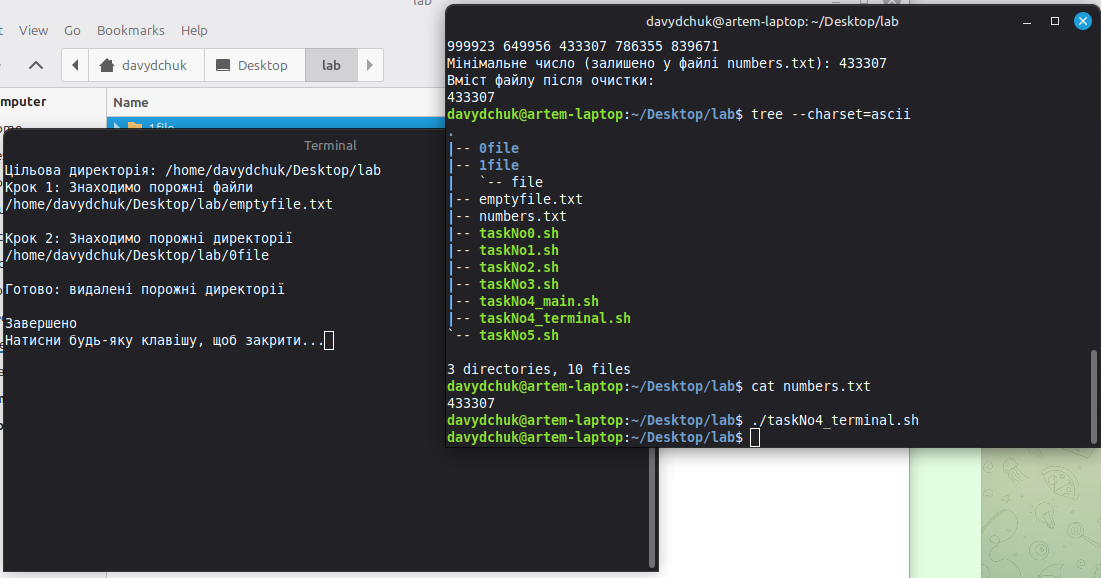
\includegraphics[width=1.0\textwidth]{task4.png}
        % Підпис (зазвичай під малюнком):
        \caption{Фото демонстрації відкриття нового вікна термінала}
        % Мітка для посилань у тексті (\ref{fig:...})
        \label{fig1:task4photo}

    \end{figure}

    \begin{minted}{bash}
davydchuk@artem-laptop:~/Desktop/lab$ tree --charset=ascii
.
|-- 1file
|   `-- file
|-- numbers.txt
|-- taskNo0.sh
|-- taskNo1.sh
|-- taskNo2.sh
|-- taskNo3.sh
|-- taskNo4_main.sh
|-- taskNo4_terminal.sh
`-- taskNo5.sh

2 directories, 9 files
    \end{minted}

    Звідси видно, що дійсно видалився файл \texttt{emptyfile.txt} і пуста директорія \texttt{0file}.

    \vspace{1em}

    Код 6 скрипта (\texttt{taskNo5.sh}):

    \begin{minted}{bash}
#!/usr/bin/env bash
# taskNo5.sh - записати в файл вивід top і залишити лише перші n рядків
set -euo pipefail

N="${1:-5}"
OUT="${2:-./top.txt}"

# Перевірка N: додатне ціле
[[ $N =~ ^[1-9][0-9]*$ ]] || { echo "Помилка: n має бути додатним цілим" >&2; exit 1; }

# 1) Повний знімок top
top -b -n1 > "$OUT"

# 2) Залишити лише перші N рядків (через тимчасовий файл - просто і прозоро)
tmp="$(mktemp "${OUT%.txt}.XXXXXX")"
head -n "$N" "$OUT" > "$tmp"
mv -f -- "$tmp" "$OUT"

echo "Записано у $OUT лише перші $N рядків виводу top"
    \end{minted}

    Перевірка:

    \begin{minted}{bash}
davydchuk@artem-laptop:~/Desktop/lab$ ./taskNo5.sh
Записано у ./top.txt лише перші 5 рядків виводу top
davydchuk@artem-laptop:~/Desktop/lab$ cat top.txt
top - 04:54:17 up  3:17,  1 user,  load average: 3,20, 1,51, 0,92
Tasks: 202 total,   1 running, 201 sleeping,   0 stopped,   0 zombie
%Cpu(s): 34,6 us, 19,2 sy,  0,0 ni, 46,2 id,  0,0 wa,  0,0 hi,  0,0 si,  0,0 st 
MiB Mem :   3915,9 total,    604,2 free,   2196,1 used,   1429,5 buff/cache     
MiB Swap:   2680,0 total,   2680,0 free,      0,0 used.   1719,7 avail Mem 
davydchuk@artem-laptop:~/Desktop/lab$ ./taskNo5.sh 15
Записано у ./top.txt лише перші 15 рядків виводу top
davydchuk@artem-laptop:~/Desktop/lab$ cat top.txt
top - 04:54:35 up  3:18,  1 user,  load average: 2,64, 1,49, 0,93
Tasks: 202 total,   3 running, 199 sleeping,   0 stopped,   0 zombie
%Cpu(s): 27,3 us, 18,2 sy,  0,0 ni, 54,5 id,  0,0 wa,  0,0 hi,  0,0 si,  0,0 st 
MiB Mem :   3915,9 total,    596,0 free,   2204,2 used,   1429,5 buff/cache     
MiB Swap:   2680,0 total,   2680,0 free,      0,0 used.   1711,6 avail Mem 

    PID USER      PR  NI    VIRT    RES    SHR S  %CPU  %MEM     TIME+ COMMAND
   1397 davydch+  20   0 4899492 324036 153548 R 158,3   8,1  54:05.86 cinnamon
   2192 davydch+  20   0   11,4g 599140 226544 S  33,3  14,9  18:46.10 firefox+
    897 root      20   0  525452 261032  83560 R  16,7   6,5   8:13.88 Xorg
   2403 davydch+  20   0   19,0g 397092 121416 S  16,7   9,9  17:55.97 Isolate+
      1 root      20   0   22408  13024   9184 S   0,0   0,3   0:01.79 systemd
      2 root      20   0       0      0      0 S   0,0   0,0   0:00.01 kthreadd
      3 root      20   0       0      0      0 S   0,0   0,0   0:00.00 pool_wo+
      4 root       0 -20       0      0      0 I   0,0   0,0   0:00.00 kworker+
    \end{minted}

    \textbf{\underline{Висновок:}} Реалізовано bash-скрипти для перевірки двох параметрів і
    виводу alias/розміру скрипта; визначення трьох найважчих директорій; проходження по вмісту теки з переміщенням файлів у
    \texttt{<name>\_dir}; генерації 5 випадкових чисел із залишенням мінімального; рекурсивного очищення порожніх файлів і
    тек та запуску в новому терміналі; знімка top з обрізанням до перших $n$ рядків;
    Демонстрація виводу результатів виконання цих скриптів підтвердила їх правильну реалізацію.

  \newpage

  \begin{titlepage}

      \begin{center}
    \phantomsection\label{sec:section4}%
    \textbf{\Large 4. РОЗДІЛ 4}
  \end{center}

        % Картинка шапки (по центру, з відступом від верху)
        \begin{center}
\includegraphics[width=0.7\textwidth]{../../../TITLES/letterhead.png}\end{center}

        \begin{center}
            \large Національний технічний університет України\\
            «Київський політехнічний інститут імені Ігоря Сікорського»\\[1em]
            Факультет інформатики та обчислювальної техніки\\
            Кафедра обчислювальної техніки
        \end{center}

        \vfill

        \begin{center}
            \textbf{\LARGE Вступ до операційної системи Linux. Курсова робота}\\[1.5em]
            \textbf{\Large Практична робота №4}\\[1em]
            «Вивчення CI/CD інстументів»
        \end{center}

        \vfill

        \begin{flushright}
            Виконав: студент 2 курсу ФІОТ, гр. ІО-41\\
            \textit{Давидчук А.~М.}\\[1em]
            Перевірив: \textit{Нікольський С.~С.}
        \end{flushright}

        \vfill

        \begin{center}Київ --- 2025\end{center}

    \end{titlepage}

    % Основний документ:

    \setlength{\parindent}{0em}

    \textbf{\underline{Тема:}} «Вивчення CI/CD інстументів».

    \vspace{1em}

    \textbf{\underline{Мета:}} навчитись користуванню інструментів CI/CD інструментів на основі Jenkins.

    \vspace{1em}

    \begin{center} \textbf{\Large Практична частина} \end{center}

    \textbf{\underline{Робоча директорія:}}

    \begin{minted}{text}
PS C:\Users\artem\Desktop\project> tree /f /a 
Folder PATH listing
Volume serial number is 1A5B-F8AF
C:.
|   .gitignore
|   CMakeLists.txt
|   
+---src
|       sort.cpp
|       sort.h
|       stringProcessor.cpp
|       stringProcessor.h
|       
\---tests
        smoke_test.cpp
    \end{minted}

    \textbf{\underline{Програмний код src/sort.cpp:}}

    \begin{minted}{cpp}
#include "sort.h"

namespace algo {

void insertion_sort(std::vector<int>& a) {
    for (size_t i = 1; i < a.size(); ++i) {
        int key = a[i];
        size_t j = i;
        while (j > 0 && a[j - 1] > key) {
            a[j] = a[j - 1];
            --j;
        }
        a[j] = key;
    }
}

bool is_sorted_non_decreasing(const std::vector<int>& a) {
    for (size_t i = 1; i < a.size(); ++i) {
        if (a[i - 1] > a[i]) return false;
    }
    return true;
}

} // namespace algo
    \end{minted}

    \newpage

    \textbf{\underline{Програмний код src/sort.h:}}

    \begin{minted}{cpp}
#pragma once
#include <vector>

namespace algo {
    // Стабільне просте сортування (in-place) — для прикладу
    void insertion_sort(std::vector<int>& a);

    // Перевірка відсортованості за нестрогим зростанням
    bool is_sorted_non_decreasing(const std::vector<int>& a);
}
    \end{minted}

    \textbf{\underline{Програмний код src/stringProcessor.cpp:}}

    \begin{minted}{cpp}
#include "stringProcessor.h"

namespace {
    inline bool is_space(char c) {
        return c == ' ' || c == '\t' || c == '\n' || c == '\r';
    }
}

namespace sp {

std::string trim(const std::string& s) {
    if (s.empty()) return s;
    size_t i = 0, j = s.size();
    while (i < j && is_space(s[i])) ++i;
    while (j > i && is_space(s[j - 1])) --j;
    return s.substr(i, j - i);
}

std::string to_lower(std::string s) {
    for (auto& c : s) {
        if (c >= 'A' && c <= 'Z') c = char(c - 'A' + 'a');
    }
    return s;
}

bool is_palindrome(const std::string& s) {
    // ігноруємо пробіли, нечутливість до регістру
    std::string t;
    t.reserve(s.size());
    for (char c : s) {
        if (!is_space(c)) t.push_back(c);
    }
    t = to_lower(t);
    size_t i = 0, j = t.size();
    if (j == 0) return true;
    --j;
    while (i < j) {
        if (t[i] != t[j]) return false;
        ++i; --j;
    }
    return true;
}

} // namespace sp
    \end{minted}

    \textbf{\underline{Програмний код src/stringProcessor.h:}}

    \begin{minted}{cpp}
#pragma once
#include <string>
#include <algorithm>

namespace sp {
    // Трим пробіли з обох боків
    std::string trim(const std::string& s);

    // До нижнього регістру (ASCII)
    std::string to_lower(std::string s);

    // Чи паліндром (без урахування регістру і пробілів)
    bool is_palindrome(const std::string& s);
}
    \end{minted}

    \textbf{\underline{Конфігурація + генерація Solution (.sln):}}

    \begin{minted}{text}
PS C:\Users\artem\Desktop\project> cmake -S . -B build -G "Visual Studio 17 2022"
-- Selecting Windows SDK version 10.0.26100.0 to target Windows 6.2.9200.
-- The CXX compiler identification is MSVC 19.44.35219.0
-- Detecting CXX compiler ABI info
-- Detecting CXX compiler ABI info - done
-- Check for working CXX compiler: C:/Program Files (x86)/Microsoft Visual Studio/2022/BuildTools/VC/Tools/MSVC/14.44.35207/bin/Hostx64/x64/cl.exe - skipped
-- Detecting CXX compile features
-- Detecting CXX compile features - done
CMake Warning (dev) at C:/Strawberry/c/share/cmake-3.29/Modules/FetchContent.cmake:1352 (message):
  The DOWNLOAD_EXTRACT_TIMESTAMP option was not given and policy CMP0135 is
  not set.  The policy's OLD behavior will be used.  When using a URL
  download, the timestamps of extracted files should preferably be that of
  the time of extraction, otherwise code that depends on the extracted
  contents might not be rebuilt if the URL changes.  The OLD behavior
  preserves the timestamps from the archive instead, but this is usually not
  what you want.  Update your project to the NEW behavior or specify the
  DOWNLOAD_EXTRACT_TIMESTAMP option with a value of true to avoid this
  robustness issue.
Call Stack (most recent call first):
  CMakeLists.txt:17 (FetchContent_Declare)
This warning is for project developers.  Use -Wno-dev to suppress it.

-- The C compiler identification is MSVC 19.44.35219.0
-- Detecting C compiler ABI info
-- Detecting C compiler ABI info - done
-- Check for working C compiler: C:/Program Files (x86)/Microsoft Visual Studio/2022/BuildTools/VC/Tools/MSVC/14.44.35207/bin/Hostx64/x64/cl.exe - skipped
-- Detecting C compile features
-- Detecting C compile features - done
-- Found Python3: C:/Users/artem/AppData/Local/Programs/Python/Python313/python.exe (found version "3.13.6") found components: Interpreter
-- Performing Test CMAKE_HAVE_LIBC_PTHREAD
-- Performing Test CMAKE_HAVE_LIBC_PTHREAD - Failed
-- Looking for pthread_create in pthreads
-- Looking for pthread_create in pthreads - not found
-- Looking for pthread_create in pthread
-- Looking for pthread_create in pthread - not found
-- Found Threads: TRUE
-- Configuring done (22.1s)
-- Generating done (0.2s)
-- Build files have been written to: C:/Users/artem/Desktop/project/build
    \end{minted}

    \textbf{\underline{Збірка (Debug):}}

    \begin{minted}{text}
PS C:\Users\artem\Desktop\project> cmake --build build --config Debug
MSBuild version 17.14.23+b0019275e for .NET Framework

  1>Checking Build System
  Building Custom Rule C:/Users/artem/Desktop/project/build/_deps/googletest-src/googlemock/
CMakeLists.txt
  gtest-all.cc
  gmock-all.cc
  Generating Code...
  gmock.vcxproj -> C:\Users\artem\Desktop\project\build\lib\Debug\gmock.lib
  Building Custom Rule C:/Users/artem/Desktop/project/build/_deps/googletest-src/googlemock/
CMakeLists.txt
  gtest-all.cc
  gmock-all.cc
  gmock_main.cc
  Generating Code...
  gmock_main.vcxproj -> C:\Users\artem\Desktop\project\build\lib\Debug\gmock_main.lib
  Building Custom Rule C:/Users/artem/Desktop/project/build/_deps/googletest-src/googletest/
CMakeLists.txt
  gtest-all.cc
  gtest.vcxproj -> C:\Users\artem\Desktop\project\build\lib\Debug\gtest.lib
  Building Custom Rule C:/Users/artem/Desktop/project/build/_deps/googletest-src/googletest/
CMakeLists.txt
  gtest_main.cc
  gtest_main.vcxproj -> C:\Users\artem\Desktop\project\build\lib\Debug\gtest_main.lib
  Building Custom Rule C:/Users/artem/Desktop/project/CMakeLists.txt
  stringProcessor.cpp
  sort.cpp
  Generating Code...
  my_lib.vcxproj -> C:\Users\artem\Desktop\project\build\Debug\my_lib.lib
  Building Custom Rule C:/Users/artem/Desktop/project/CMakeLists.txt
  smoke_test.cpp
  unit_tests.vcxproj -> C:\Users\artem\Desktop\project\build\Debug\unit_tests.exe
  Building Custom Rule C:/Users/artem/Desktop/project/CMakeLists.txt
    \end{minted}

    \textbf{\underline{Запуск тестів з генерацією XML-звіту}}:

    \begin{minted}{text}
PS C:\Users\artem\Desktop\project> .\build\Debug\unit_tests.exe --gtest_output=xml:build\test_report.xml
Running main() from C:\Users\artem\Desktop\project\build\_deps\googletest-src\googletest\src
gtest_main.cc
[==========] Running 3 tests from 2 test suites.
[----------] Global test environment set-up.
[----------] 2 tests from StringProcessor
[ RUN      ] StringProcessor.TrimAndLower
[       OK ] StringProcessor.TrimAndLower (0 ms)
[ RUN      ] StringProcessor.Palindrome
[       OK ] StringProcessor.Palindrome (0 ms)
[----------] 2 tests from StringProcessor (1 ms total)

[----------] 1 test from Sort
[ RUN      ] Sort.InsertionSortWorks
[       OK ] Sort.InsertionSortWorks (0 ms)
[----------] 1 test from Sort (0 ms total)

[----------] Global test environment tear-down
[==========] 3 tests from 2 test suites ran. (4 ms total)
[  PASSED  ] 3 tests.
    \end{minted}

    \textbf{\underline{Робоча директорія після виконаних кроків конфігурації, генерації та збірки:}}

    \begin{minted}{text}
PS C:\Users\artem\Desktop\project> tree /f /a
Folder PATH listing
Volume serial number is 1A5B-F8AF
C:.
|   .consolestory
|   .gitignore
|   CMakeLists.txt
|   t.txt
|   
+---build
|   |   ALL_BUILD.vcxproj
|   |   ALL_BUILD.vcxproj.filters
|   |   CMakeCache.txt
|   |   cmake_install.cmake
|   |   CTestTestfile.cmake
|   |   INSTALL.vcxproj
|   |   INSTALL.vcxproj.filters
|   |   MyGTestProj.sln
|   |   my_lib.vcxproj
|   |   my_lib.vcxproj.filters
|   |   RUN_TESTS.vcxproj
|   |   RUN_TESTS.vcxproj.filters
|   |   test_report.xml
|   |   unit_tests.vcxproj
|   |   unit_tests.vcxproj.filters
|   |   unit_tests[1]_include.cmake
|   |   unit_tests[1]_tests.cmake
|   |   ZERO_CHECK.vcxproj
|   |   ZERO_CHECK.vcxproj.filters
|   |   
|   +---CMakeFiles
|   |   |   cmake.check_cache
|   |   |   CMakeConfigureLog.yaml
|   |   |   generate.stamp
|   |   |   generate.stamp.depend
|   |   |   generate.stamp.list
|   |   |   TargetDirectories.txt
|   |   |   
|   |   +---221e8778a9cacabaa0e7dca956df043d
|   |   |       INSTALL_force.rule
|   |   |       RUN_TESTS_force.rule
|   |   |       
|   |   +---3.29.2
|   |   |   |   CMakeCCompiler.cmake
|   |   |   |   CMakeCXXCompiler.cmake
|   |   |   |   CMakeDetermineCompilerABI_C.bin
|   |   |   |   CMakeDetermineCompilerABI_CXX.bin
|   |   |   |   CMakeRCCompiler.cmake
|   |   |   |   CMakeSystem.cmake
|   |   |   |   VCTargetsPath.txt
|   |   |   |   VCTargetsPath.vcxproj
|   |   |   |   
|   |   |   +---CompilerIdC
|   |   |   |   |   CMakeCCompilerId.c
|   |   |   |   |   CompilerIdC.exe
|   |   |   |   |   CompilerIdC.vcxproj
|   |   |   |   |   
|   |   |   |   +---Debug
|   |   |   |   |   |   CMakeCCompilerId.obj
|   |   |   |   |   |   CompilerIdC.exe.recipe
|   |   |   |   |   |   
|   |   |   |   |   \---CompilerIdC.tlog
|   |   |   |   |           CL.command.1.tlog
|   |   |   |   |           Cl.items.tlog
|   |   |   |   |           CL.read.1.tlog
|   |   |   |   |           CL.write.1.tlog
|   |   |   |   |           CompilerIdC.lastbuildstate
|   |   |   |   |           link.command.1.tlog
|   |   |   |   |           link.read.1.tlog
|   |   |   |   |           link.secondary.1.tlog
|   |   |   |   |           link.write.1.tlog
|   |   |   |   |           
|   |   |   |   \---tmp
|   |   |   +---CompilerIdCXX
|   |   |   |   |   CMakeCXXCompilerId.cpp
|   |   |   |   |   CompilerIdCXX.exe
|   |   |   |   |   CompilerIdCXX.vcxproj
|   |   |   |   |   
|   |   |   |   +---Debug
|   |   |   |   |   |   CMakeCXXCompilerId.obj
|   |   |   |   |   |   CompilerIdCXX.exe.recipe
|   |   |   |   |   |   
|   |   |   |   |   \---CompilerIdCXX.tlog
|   |   |   |   |           CL.command.1.tlog
|   |   |   |   |           Cl.items.tlog
|   |   |   |   |           CL.read.1.tlog
|   |   |   |   |           CL.write.1.tlog
|   |   |   |   |           CompilerIdCXX.lastbuildstate
|   |   |   |   |           link.command.1.tlog
|   |   |   |   |           link.read.1.tlog
|   |   |   |   |           link.secondary.1.tlog
|   |   |   |   |           link.write.1.tlog
|   |   |   |   |           
|   |   |   |   \---tmp
|   |   |   +---VCTargetsPath
|   |   |   |   \---x64
|   |   |   |       \---Debug
|   |   |   |           |   VCTargetsPath.recipe
|   |   |   |           |   
|   |   |   |           \---VCTargetsPath.tlog
|   |   |   |                   VCTargetsPath.lastbuildstate
|   |   |   |                   
|   |   |   \---x64
|   |   |       \---Debug
|   |   +---ba30693984164defdda498b2fc47b999
|   |   |       generate.stamp.rule
|   |   |       INSTALL_force.rule
|   |   |       RUN_TESTS_force.rule
|   |   |       
|   |   +---CMakeScratch
|   |   +---e1016b5e72a78186d6d2c7373e841be2
|   |   |       INSTALL_force.rule
|   |   |       RUN_TESTS_force.rule
|   |   |       
|   |   +---e5097ab0b0bc71e539ee0b41c04d6012
|   |   |       INSTALL_force.rule
|   |   |       RUN_TESTS_force.rule
|   |   |       
|   |   \---pkgRedirects
|   +---Debug
|   |       my_lib.lib
|   |       my_lib.pdb
|   |       unit_tests.exe
|   |       unit_tests.pdb
|   |       
|   +---lib
|   |   \---Debug
|   |           gmock.lib
|   |           gmock.pdb
|   |           gmockpdb_debug_postfix-NOTFOUND.pdb
|   |           gmock_main.lib
|   |           gmock_main.pdb
|   |           gmock_mainpdb_debug_postfix-NOTFOUND.pdb
|   |           gtest.lib
|   |           gtest.pdb
|   |           gtestpdb_debug_postfix-NOTFOUND.pdb
|   |           gtest_main.lib
|   |           gtest_main.pdb
|   |           gtest_mainpdb_debug_postfix-NOTFOUND.pdb
|   |           
|   +---my_lib.dir
|   |   \---Debug
|   |       |   my_lib.lib.recipe
|   |       |   sort.obj
|   |       |   stringProcessor.obj
|   |       |   
|   |       \---my_lib.tlog
|   |               CL.command.1.tlog
|   |               Cl.items.tlog
|   |               CL.read.1.tlog
|   |               CL.write.1.tlog
|   |               CustomBuild.command.1.tlog
|   |               CustomBuild.read.1.tlog
|   |               CustomBuild.write.1.tlog
|   |               Lib-link.read.1.tlog
|   |               Lib-link.write.1.tlog
|   |               Lib.command.1.tlog
|   |               my_lib.lastbuildstate
|   |               
|   +---unit_tests.dir
|   |   \---Debug
|   |       |   smoke_test.obj
|   |       |   unit_tests.exe.recipe
|   |       |   unit_tests.ilk
|   |       |   vc143.pdb
|   |       |   
|   |       \---unit_tests.tlog
|   |               CL.command.1.tlog
|   |               Cl.items.tlog
|   |               CL.read.1.tlog
|   |               CL.write.1.tlog
|   |               CustomBuild.command.1.tlog
|   |               CustomBuild.read.1.tlog
|   |               CustomBuild.write.1.tlog
|   |               link.command.1.tlog
|   |               link.read.1.tlog
|   |               link.secondary.1.tlog
|   |               link.write.1.tlog
|   |               unit_tests.lastbuildstate
|   |               
|   +---x64
|   |   \---Debug
|   |       +---ALL_BUILD
|   |       |   |   ALL_BUILD.recipe
|   |       |   |   
|   |       |   \---ALL_BUILD.tlog
|   |       |           ALL_BUILD.lastbuildstate
|   |       |           CustomBuild.command.1.tlog
|   |       |           CustomBuild.read.1.tlog
|   |       |           CustomBuild.write.1.tlog
|   |       |           
|   |       \---ZERO_CHECK
|   |           |   ZERO_CHECK.recipe
|   |           |   
|   |           \---ZERO_CHECK.tlog
|   |                   CustomBuild.command.1.tlog
|   |                   CustomBuild.read.1.tlog
|   |                   CustomBuild.write.1.tlog
|   |                   ZERO_CHECK.lastbuildstate
|   |                   
|   \---_deps
|       +---googletest-build
|       |   |   ALL_BUILD.vcxproj
|       |   |   ALL_BUILD.vcxproj.filters
|       |   |   cmake_install.cmake
|       |   |   CTestTestfile.cmake
|       |   |   googletest-distribution.sln
|       |   |   INSTALL.vcxproj
|       |   |   INSTALL.vcxproj.filters
|       |   |   RUN_TESTS.vcxproj
|       |   |   RUN_TESTS.vcxproj.filters
|       |   |   
|       |   +---CMakeFiles
|       |   |       generate.stamp
|       |   |       generate.stamp.depend
|       |   |       
|       |   +---googlemock
|       |   |   |   ALL_BUILD.vcxproj
|       |   |   |   ALL_BUILD.vcxproj.filters
|       |   |   |   cmake_install.cmake
|       |   |   |   CTestTestfile.cmake
|       |   |   |   gmock.sln
|       |   |   |   gmock.vcxproj
|       |   |   |   gmock.vcxproj.filters
|       |   |   |   gmock_main.vcxproj
|       |   |   |   gmock_main.vcxproj.filters
|       |   |   |   INSTALL.vcxproj
|       |   |   |   INSTALL.vcxproj.filters
|       |   |   |   RUN_TESTS.vcxproj
|       |   |   |   RUN_TESTS.vcxproj.filters
|       |   |   |   
|       |   |   +---CMakeFiles
|       |   |   |       generate.stamp
|       |   |   |       generate.stamp.depend
|       |   |   |       
|       |   |   +---gmock.dir
|       |   |   |   \---Debug
|       |   |   |       |   gmock-all.obj
|       |   |   |       |   gmock.lib.recipe
|       |   |   |       |   gtest-all.obj
|       |   |   |       |   
|       |   |   |       \---gmock.tlog
|       |   |   |               CL.command.1.tlog
|       |   |   |               Cl.items.tlog
|       |   |   |               CL.read.1.tlog
|       |   |   |               CL.write.1.tlog
|       |   |   |               CustomBuild.command.1.tlog
|       |   |   |               CustomBuild.read.1.tlog
|       |   |   |               CustomBuild.write.1.tlog
|       |   |   |               gmock.lastbuildstate
|       |   |   |               Lib-link.read.1.tlog
|       |   |   |               Lib-link.write.1.tlog
|       |   |   |               Lib.command.1.tlog
|       |   |   |               
|       |   |   \---gmock_main.dir
|       |   |       \---Debug
|       |   |           |   gmock-all.obj
|       |   |           |   gmock_main.lib.recipe
|       |   |           |   gmock_main.obj
|       |   |           |   gtest-all.obj
|       |   |           |   
|       |   |           \---gmock_main.tlog
|       |   |                   CL.command.1.tlog
|       |   |                   Cl.items.tlog
|       |   |                   CL.read.1.tlog
|       |   |                   CL.write.1.tlog
|       |   |                   CustomBuild.command.1.tlog
|       |   |                   CustomBuild.read.1.tlog
|       |   |                   CustomBuild.write.1.tlog
|       |   |                   gmock_main.lastbuildstate
|       |   |                   Lib-link.read.1.tlog
|       |   |                   Lib-link.write.1.tlog
|       |   |                   Lib.command.1.tlog
|       |   |                   
|       |   \---googletest
|       |       |   ALL_BUILD.vcxproj
|       |       |   ALL_BUILD.vcxproj.filters
|       |       |   cmake_install.cmake
|       |       |   CTestTestfile.cmake
|       |       |   gtest.sln
|       |       |   gtest.vcxproj
|       |       |   gtest.vcxproj.filters
|       |       |   gtest_main.vcxproj
|       |       |   gtest_main.vcxproj.filters
|       |       |   INSTALL.vcxproj
|       |       |   INSTALL.vcxproj.filters
|       |       |   RUN_TESTS.vcxproj
|       |       |   RUN_TESTS.vcxproj.filters
|       |       |   
|       |       +---CMakeFiles
|       |       |   |   generate.stamp
|       |       |   |   generate.stamp.depend
|       |       |   |   
|       |       |   \---Export
|       |       |       \---0c08b8e77dd885bfe55a19a9659d9fc1
|       |       |               GTestTargets-debug.cmake
|       |       |               GTestTargets-minsizerel.cmake
|       |       |               GTestTargets-release.cmake
|       |       |               GTestTargets-relwithdebinfo.cmake
|       |       |               GTestTargets.cmake
|       |       |               
|       |       +---generated
|       |       |       gmock.pc
|       |       |       gmock_main.pc
|       |       |       gtest.pc
|       |       |       GTestConfig.cmake
|       |       |       GTestConfigVersion.cmake
|       |       |       gtest_main.pc
|       |       |       
|       |       +---gtest.dir
|       |       |   \---Debug
|       |       |       |   gtest-all.obj
|       |       |       |   gtest.lib.recipe
|       |       |       |   
|       |       |       \---gtest.tlog
|       |       |               CL.command.1.tlog
|       |       |               Cl.items.tlog
|       |       |               CL.read.1.tlog
|       |       |               CL.write.1.tlog
|       |       |               CustomBuild.command.1.tlog
|       |       |               CustomBuild.read.1.tlog
|       |       |               CustomBuild.write.1.tlog
|       |       |               gtest.lastbuildstate
|       |       |               Lib-link.read.1.tlog
|       |       |               Lib-link.write.1.tlog
|       |       |               Lib.command.1.tlog
|       |       |               
|       |       \---gtest_main.dir
|       |           \---Debug
|       |               |   gtest_main.lib.recipe
|       |               |   gtest_main.obj
|       |               |   
|       |               \---gtest_main.tlog
|       |                       CL.command.1.tlog
|       |                       Cl.items.tlog
|       |                       CL.read.1.tlog
|       |                       CL.write.1.tlog
|       |                       CustomBuild.command.1.tlog
|       |                       CustomBuild.read.1.tlog
|       |                       CustomBuild.write.1.tlog
|       |                       gtest_main.lastbuildstate
|       |                       Lib-link.read.1.tlog
|       |                       Lib-link.write.1.tlog
|       |                       Lib.command.1.tlog
|       |                       
|       +---googletest-src
|       |   |   .clang-format
|       |   |   .gitignore
|       |   |   BUILD.bazel
|       |   |   CMakeLists.txt
|       |   |   CONTRIBUTING.md
|       |   |   CONTRIBUTORS
|       |   |   googletest_deps.bzl
|       |   |   LICENSE
|       |   |   README.md
|       |   |   WORKSPACE
|       |   |   
|       |   +---.github
|       |   |   +---ISSUE_TEMPLATE
|       |   |   |       00-bug_report.yml
|       |   |   |       10-feature_request.yml
|       |   |   |       config.yml
|       |   |   |       
|       |   |   \---workflows
|       |   |           gtest-ci.yml
|       |   |           
|       |   +---ci
|       |   |       linux-presubmit.sh
|       |   |       macos-presubmit.sh
|       |   |       windows-presubmit.bat
|       |   |       
|       |   +---docs
|       |   |   |   advanced.md
|       |   |   |   community_created_documentation.md
|       |   |   |   faq.md
|       |   |   |   gmock_cheat_sheet.md
|       |   |   |   gmock_cook_book.md
|       |   |   |   gmock_faq.md
|       |   |   |   gmock_for_dummies.md
|       |   |   |   index.md
|       |   |   |   pkgconfig.md
|       |   |   |   platforms.md
|       |   |   |   primer.md
|       |   |   |   quickstart-bazel.md
|       |   |   |   quickstart-cmake.md
|       |   |   |   samples.md
|       |   |   |   _config.yml
|       |   |   |   
|       |   |   +---assets
|       |   |   |   \---css
|       |   |   |           style.scss
|       |   |   |           
|       |   |   +---reference
|       |   |   |       actions.md
|       |   |   |       assertions.md
|       |   |   |       matchers.md
|       |   |   |       mocking.md
|       |   |   |       testing.md
|       |   |   |       
|       |   |   +---_data
|       |   |   |       navigation.yml
|       |   |   |       
|       |   |   +---_layouts
|       |   |   |       default.html
|       |   |   |       
|       |   |   \---_sass
|       |   |           main.scss
|       |   |           
|       |   +---googlemock
|       |   |   |   CMakeLists.txt
|       |   |   |   README.md
|       |   |   |   
|       |   |   +---cmake
|       |   |   |       gmock.pc.in
|       |   |   |       gmock_main.pc.in
|       |   |   |       
|       |   |   +---docs
|       |   |   |       README.md
|       |   |   |       
|       |   |   +---include
|       |   |   |   \---gmock
|       |   |   |       |   gmock-actions.h
|       |   |   |       |   gmock-cardinalities.h
|       |   |   |       |   gmock-function-mocker.h
|       |   |   |       |   gmock-matchers.h
|       |   |   |       |   gmock-more-actions.h
|       |   |   |       |   gmock-more-matchers.h
|       |   |   |       |   gmock-nice-strict.h
|       |   |   |       |   gmock-spec-builders.h
|       |   |   |       |   gmock.h
|       |   |   |       |   
|       |   |   |       \---internal
|       |   |   |           |   gmock-internal-utils.h
|       |   |   |           |   gmock-port.h
|       |   |   |           |   gmock-pp.h
|       |   |   |           |   
|       |   |   |           \---custom
|       |   |   |                   gmock-generated-actions.h
|       |   |   |                   gmock-matchers.h
|       |   |   |                   gmock-port.h
|       |   |   |                   README.md
|       |   |   |                   
|       |   |   +---src
|       |   |   |       gmock-all.cc
|       |   |   |       gmock-cardinalities.cc
|       |   |   |       gmock-internal-utils.cc
|       |   |   |       gmock-matchers.cc
|       |   |   |       gmock-spec-builders.cc
|       |   |   |       gmock.cc
|       |   |   |       gmock_main.cc
|       |   |   |       
|       |   |   \---test
|       |   |           BUILD.bazel
|       |   |           gmock-actions_test.cc
|       |   |           gmock-cardinalities_test.cc
|       |   |           gmock-function-mocker_test.cc
|       |   |           gmock-internal-utils_test.cc
|       |   |           gmock-matchers-arithmetic_test.cc
|       |   |           gmock-matchers-comparisons_test.cc
|       |   |           gmock-matchers-containers_test.cc
|       |   |           gmock-matchers-misc_test.cc
|       |   |           gmock-matchers_test.h
|       |   |           gmock-more-actions_test.cc
|       |   |           gmock-nice-strict_test.cc
|       |   |           gmock-port_test.cc
|       |   |           gmock-pp-string_test.cc
|       |   |           gmock-pp_test.cc
|       |   |           gmock-spec-builders_test.cc
|       |   |           gmock_all_test.cc
|       |   |           gmock_ex_test.cc
|       |   |           gmock_leak_test.py
|       |   |           gmock_leak_test_.cc
|       |   |           gmock_link2_test.cc
|       |   |           gmock_link_test.cc
|       |   |           gmock_link_test.h
|       |   |           gmock_output_test.py
|       |   |           gmock_output_test_.cc
|       |   |           gmock_output_test_golden.txt
|       |   |           gmock_stress_test.cc
|       |   |           gmock_test.cc
|       |   |           gmock_test_utils.py
|       |   |           
|       |   \---googletest
|       |       |   CMakeLists.txt
|       |       |   README.md
|       |       |   
|       |       +---cmake
|       |       |       Config.cmake.in
|       |       |       gtest.pc.in
|       |       |       gtest_main.pc.in
|       |       |       internal_utils.cmake
|       |       |       libgtest.la.in
|       |       |       
|       |       +---docs
|       |       |       README.md
|       |       |       
|       |       +---include
|       |       |   \---gtest
|       |       |       |   gtest-assertion-result.h
|       |       |       |   gtest-death-test.h
|       |       |       |   gtest-matchers.h
|       |       |       |   gtest-message.h
|       |       |       |   gtest-param-test.h
|       |       |       |   gtest-printers.h
|       |       |       |   gtest-spi.h
|       |       |       |   gtest-test-part.h
|       |       |       |   gtest-typed-test.h
|       |       |       |   gtest.h
|       |       |       |   gtest_pred_impl.h
|       |       |       |   gtest_prod.h
|       |       |       |   
|       |       |       \---internal
|       |       |           |   gtest-death-test-internal.h
|       |       |           |   gtest-filepath.h
|       |       |           |   gtest-internal.h
|       |       |           |   gtest-param-util.h
|       |       |           |   gtest-port-arch.h
|       |       |           |   gtest-port.h
|       |       |           |   gtest-string.h
|       |       |           |   gtest-type-util.h
|       |       |           |   
|       |       |           \---custom
|       |       |                   gtest-port.h
|       |       |                   gtest-printers.h
|       |       |                   gtest.h
|       |       |                   README.md
|       |       |                   
|       |       +---samples
|       |       |       prime_tables.h
|       |       |       sample1.cc
|       |       |       sample1.h
|       |       |       sample10_unittest.cc
|       |       |       sample1_unittest.cc
|       |       |       sample2.cc
|       |       |       sample2.h
|       |       |       sample2_unittest.cc
|       |       |       sample3-inl.h
|       |       |       sample3_unittest.cc
|       |       |       sample4.cc
|       |       |       sample4.h
|       |       |       sample4_unittest.cc
|       |       |       sample5_unittest.cc
|       |       |       sample6_unittest.cc
|       |       |       sample7_unittest.cc
|       |       |       sample8_unittest.cc
|       |       |       sample9_unittest.cc
|       |       |       
|       |       +---src
|       |       |       gtest-all.cc
|       |       |       gtest-assertion-result.cc
|       |       |       gtest-death-test.cc
|       |       |       gtest-filepath.cc
|       |       |       gtest-internal-inl.h
|       |       |       gtest-matchers.cc
|       |       |       gtest-port.cc
|       |       |       gtest-printers.cc
|       |       |       gtest-test-part.cc
|       |       |       gtest-typed-test.cc
|       |       |       gtest.cc
|       |       |       gtest_main.cc
|       |       |       
|       |       \---test
|       |               BUILD.bazel
|       |               googletest-break-on-failure-unittest.py
|       |               googletest-break-on-failure-unittest_.cc
|       |               googletest-catch-exceptions-test.py
|       |               googletest-catch-exceptions-test_.cc
|       |               googletest-color-test.py
|       |               googletest-color-test_.cc
|       |               googletest-death-test-test.cc
|       |               googletest-death-test_ex_test.cc
|       |               googletest-env-var-test.py
|       |               googletest-env-var-test_.cc
|       |               googletest-failfast-unittest.py
|       |               googletest-failfast-unittest_.cc
|       |               googletest-filepath-test.cc
|       |               googletest-filter-unittest.py
|       |               googletest-filter-unittest_.cc
|       |               googletest-global-environment-unittest.py
|       |               googletest-global-environment-unittest_.cc
|       |               googletest-json-outfiles-test.py
|       |               googletest-json-output-unittest.py
|       |               googletest-list-tests-unittest.py
|       |               googletest-list-tests-unittest_.cc
|       |               googletest-listener-test.cc
|       |               googletest-message-test.cc
|       |               googletest-options-test.cc
|       |               googletest-output-test-golden-lin.txt
|       |               googletest-output-test.py
|       |               googletest-output-test_.cc
|       |               googletest-param-test-invalid-name1-test.py
|       |               googletest-param-test-invalid-name1-test_.cc
|       |               googletest-param-test-invalid-name2-test.py
|       |               googletest-param-test-invalid-name2-test_.cc
|       |               googletest-param-test-test.cc
|       |               googletest-param-test-test.h
|       |               googletest-param-test2-test.cc
|       |               googletest-port-test.cc
|       |               googletest-printers-test.cc
|       |               googletest-setuptestsuite-test.py
|       |               googletest-setuptestsuite-test_.cc
|       |               googletest-shuffle-test.py
|       |               googletest-shuffle-test_.cc
|       |               googletest-test-part-test.cc
|       |               googletest-throw-on-failure-test.py
|       |               googletest-throw-on-failure-test_.cc
|       |               googletest-uninitialized-test.py
|       |               googletest-uninitialized-test_.cc
|       |               gtest-typed-test2_test.cc
|       |               gtest-typed-test_test.cc
|       |               gtest-typed-test_test.h
|       |               gtest-unittest-api_test.cc
|       |               gtest_all_test.cc
|       |               gtest_assert_by_exception_test.cc
|       |               gtest_dirs_test.cc
|       |               gtest_environment_test.cc
|       |               gtest_help_test.py
|       |               gtest_help_test_.cc
|       |               gtest_json_test_utils.py
|       |               gtest_list_output_unittest.py
|       |               gtest_list_output_unittest_.cc
|       |               gtest_main_unittest.cc
|       |               gtest_no_test_unittest.cc
|       |               gtest_pred_impl_unittest.cc
|       |               gtest_premature_exit_test.cc
|       |               gtest_prod_test.cc
|       |               gtest_repeat_test.cc
|       |               gtest_skip_check_output_test.py
|       |               gtest_skip_environment_check_output_test.py
|       |               gtest_skip_in_environment_setup_test.cc
|       |               gtest_skip_test.cc
|       |               gtest_sole_header_test.cc
|       |               gtest_stress_test.cc
|       |               gtest_testbridge_test.py
|       |               gtest_testbridge_test_.cc
|       |               gtest_test_macro_stack_footprint_test.cc
|       |               gtest_test_utils.py
|       |               gtest_throw_on_failure_ex_test.cc
|       |               gtest_unittest.cc
|       |               gtest_xml_outfile1_test_.cc
|       |               gtest_xml_outfile2_test_.cc
|       |               gtest_xml_outfiles_test.py
|       |               gtest_xml_output_unittest.py
|       |               gtest_xml_output_unittest_.cc
|       |               gtest_xml_test_utils.py
|       |               production.cc
|       |               production.h
|       |               
|       \---googletest-subbuild
|           |   ALL_BUILD.vcxproj
|           |   ALL_BUILD.vcxproj.filters
|           |   CMakeCache.txt
|           |   CMakeLists.txt
|           |   cmake_install.cmake
|           |   googletest-populate.sln
|           |   googletest-populate.vcxproj
|           |   googletest-populate.vcxproj.filters
|           |   ZERO_CHECK.vcxproj
|           |   ZERO_CHECK.vcxproj.filters
|           |   
|           +---CMakeFiles
|           |   |   cmake.check_cache
|           |   |   CMakeConfigureLog.yaml
|           |   |   generate.stamp
|           |   |   generate.stamp.depend
|           |   |   generate.stamp.list
|           |   |   TargetDirectories.txt
|           |   |   
|           |   +---1df006e100ab1775d6b8844f8a1a250d
|           |   |       googletest-populate-build.rule
|           |   |       googletest-populate-configure.rule
|           |   |       googletest-populate-download.rule
|           |   |       googletest-populate-install.rule
|           |   |       googletest-populate-mkdir.rule
|           |   |       googletest-populate-patch.rule
|           |   |       googletest-populate-test.rule
|           |   |       googletest-populate-update.rule
|           |   |       
|           |   +---3.29.2
|           |   |   |   CMakeSystem.cmake
|           |   |   |   VCTargetsPath.txt
|           |   |   |   VCTargetsPath.vcxproj
|           |   |   |   
|           |   |   +---VCTargetsPath
|           |   |   |   \---x64
|           |   |   |       \---Debug
|           |   |   |           |   VCTargetsPath.recipe
|           |   |   |           |   
|           |   |   |           \---VCTargetsPath.tlog
|           |   |   |                   VCTargetsPath.lastbuildstate
|           |   |   |                   
|           |   |   \---x64
|           |   |       \---Debug
|           |   +---7e147cec0cdb2f86e12efc8064ce9745
|           |   |       googletest-populate-complete.rule
|           |   |       
|           |   +---ae8f1a22d6213c4e2d2070d31ab9c5d6
|           |   |       generate.stamp.rule
|           |   |       googletest-populate.rule
|           |   |       
|           |   +---Debug
|           |   |       googletest-populate-complete
|           |   |       
|           |   +---googletest-populate.dir
|           |   |       Labels.json
|           |   |       Labels.txt
|           |   |       
|           |   \---pkgRedirects
|           +---googletest-populate-prefix
|           |   +---src
|           |   |   |   v1.14.0.zip
|           |   |   |   
|           |   |   \---googletest-populate-stamp
|           |   |       |   download-googletest-populate.cmake
|           |   |       |   extract-googletest-populate.cmake
|           |   |       |   googletest-populate-patch-info.txt
|           |   |       |   googletest-populate-update-info.txt
|           |   |       |   googletest-populate-urlinfo.txt
|           |   |       |   verify-googletest-populate.cmake
|           |   |       |   
|           |   |       \---Debug
|           |   |               googletest-populate-build
|           |   |               googletest-populate-configure
|           |   |               googletest-populate-done
|           |   |               googletest-populate-download
|           |   |               googletest-populate-install
|           |   |               googletest-populate-mkdir
|           |   |               googletest-populate-patch
|           |   |               googletest-populate-test
|           |   |               googletest-populate-update
|           |   |               
|           |   \---tmp
|           |           googletest-populate-cfgcmd.txt
|           |           googletest-populate-mkdirs.cmake
|           |           
|           \---x64
|               \---Debug
|                   +---ALL_BUILD
|                   |   |   ALL_BUILD.recipe
|                   |   |   
|                   |   \---ALL_BUILD.tlog
|                   |           ALL_BUILD.lastbuildstate
|                   |           CustomBuild.command.1.tlog
|                   |           CustomBuild.read.1.tlog
|                   |           CustomBuild.write.1.tlog
|                   |           
|                   +---googletest-populate
|                   |   |   googletest-populate.recipe
|                   |   |   
|                   |   \---googlete.DB0C7D59.tlog
|                   |           CustomBuild.command.1.tlog
|                   |           CustomBuild.read.1.tlog
|                   |           CustomBuild.write.1.tlog
|                   |           googletest-populate.lastbuildstate
|                   |           
|                   \---ZERO_CHECK
|                       |   ZERO_CHECK.recipe
|                       |   
|                       \---ZERO_CHECK.tlog
|                               CustomBuild.command.1.tlog
|                               CustomBuild.read.1.tlog
|                               CustomBuild.write.1.tlog
|                               ZERO_CHECK.lastbuildstate
|                               
+---src
|       sort.cpp
|       sort.h
|       stringProcessor.cpp
|       stringProcessor.h
|       
\---tests
        smoke_test.cpp
    \end{minted}

    \textbf{\underline{Окремо файл build\textbackslash test$\_$report.xml:}}

    \begin{minted}{xml}
<?xml version="1.0" encoding="UTF-8"?>
<testsuites tests="3" failures="0" disabled="0" errors="0" time="0.004" timestamp="2025-11-05T16:03:04.226" name="AllTests">
  <testsuite name="StringProcessor" tests="2" failures="0" disabled="0" skipped="0" errors="0" time="0.001" timestamp="2025-11-05T16:03:04.227">
    <testcase name="TrimAndLower" file="C:\Users\artem\Desktop\project\tests\smoke_test.cpp" line="6" status="run" result="completed" time="0." timestamp="2025-11-05T16:03:04.227" classname="StringProcessor" />
    <testcase name="Palindrome" file="C:\Users\artem\Desktop\project\tests\smoke_test.cpp" line="12" status="run" result="completed" time="0." timestamp="2025-11-05T16:03:04.228" classname="StringProcessor" />
  </testsuite>
  <testsuite name="Sort" tests="1" failures="0" disabled="0" skipped="0" errors="0" time="0." timestamp="2025-11-05T16:03:04.229">
    <testcase name="InsertionSortWorks" file="C:\Users\artem\Desktop\project\tests\smoke_test.cpp" line="19" status="run" result="completed" time="0." timestamp="2025-11-05T16:03:04.229" classname="Sort" />
  </testsuite>
</testsuites>
    \end{minted}

    \textbf{\underline{Ініціалізація локального репозиторію, підключення віддаленого:}}

    \begin{minted}{text}
PS C:\Users\artem\Desktop\project> git init 
Initialized empty Git repository in C:/Users/artem/Desktop/project/.git/

PS C:\Users\artem\Desktop\project> git add .

PS C:\Users\artem\Desktop\project> git commit -m "Ініціалізація: CMake + GTest + XML Report" 
[main (root-commit) 009d10f] Ініціалізація: CMake + GTest + XML Report
 7 files changed, 174 insertions(+)
 create mode 100644 .gitignore
 create mode 100644 CMakeLists.txt
 create mode 100644 src/sort.cpp
 create mode 100644 src/sort.h
 create mode 100644 src/stringProcessor.cpp
 create mode 100644 src/stringProcessor.h
 create mode 100644 tests/smoke_test.cpp

PS C:\Users\artem\Desktop\project> git branch 
* main

PS C:\Users\artem\Desktop\project> git remote add origin https://gitea.com/davydchuk/task4lab.git

PS C:\Users\artem\Desktop\project> git push -u origin main 
Enumerating objects: 11, done.
Counting objects: 100% (11/11), done.
Delta compression using up to 16 threads
Compressing objects: 100% (10/10), done.
Writing objects: 100% (11/11), 2.88 KiB | 589.00 KiB/s, done.
Total 11 (delta 0), reused 0 (delta 0), pack-reused 0 (from 0)
remote: . Processing 1 references
remote: Processed 1 references in total
To https://gitea.com/davydchuk/task4lab.git
 * [new branch]      main -> main
branch 'main' set up to track 'origin/main'
    \end{minted}

    \textbf{\underline{Вміст Jenkinsfile:}}

    \begin{minted}{text}
pipeline {
  agent any
  stages {
    stage('Checkout') {
      steps {
        git branch: 'main',
            credentialsId: 'gitea-token-id',
            url: 'https://gitea.com/davydchuk/task4lab.git'
      }
    }
    stage('Build') {
    steps {
        bat 'cmake -S . -B build -G "Visual Studio 17 2022"'
        bat 'cmake --build build --config Debug'
    }
    }
    stage('Test') {
      steps {
        bat '.\\build\\Debug\\unit_tests.exe --gtest_output=xml:build\\test_report.xml'
      }
    }
  }
  post {
    always {
      junit 'build/test_report.xml'
    }
  }
}
    \end{minted}

    \textbf{\underline{Додаємо Jenkinsfile до віддаленого репозиторію:}}

    \begin{minted}{text}
PS C:\Users\artem\Desktop\project> git add Jenkinsfile
PS C:\Users\artem\Desktop\project> git commit -m "Додавання Jenkinsfile"  
[main 309c585] Додавання Jenkinsfile
 1 file changed, 31 insertions(+)
 create mode 100644 Jenkinsfile
PS C:\Users\artem\Desktop\project> git push 
Enumerating objects: 4, done.
Counting objects: 100% (4/4), done.
Delta compression using up to 16 threads
Compressing objects: 100% (3/3), done.
Writing objects: 100% (3/3), 792 bytes | 792.00 KiB/s, done.
Total 3 (delta 1), reused 0 (delta 0), pack-reused 0 (from 0)
remote: . Processing 1 references
remote: Processed 1 references in total
To https://gitea.com/davydchuk/task4lab.git
   009d10f..309c585  main -> main
    \end{minted}

    \textbf{\underline{Результат Unit-тестів за допомогою Jenkins:}}

    \begin{figure}[h!]
        \centering

        \begin{subfigure}{0.5\textwidth}
            \centering
            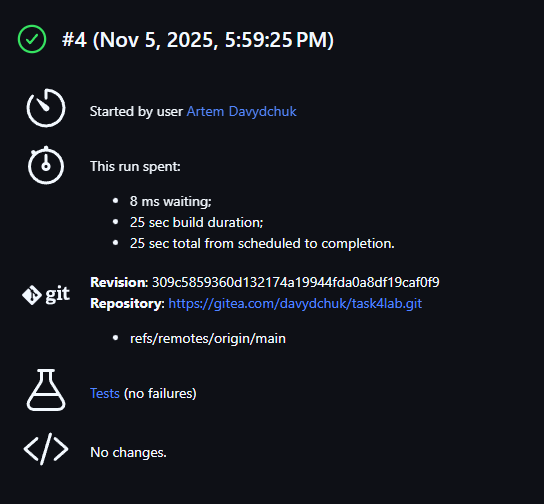
\includegraphics[width=\linewidth]{image1.png}
        \end{subfigure}\hfill
        \begin{subfigure}{0.5\textwidth}
            \centering
            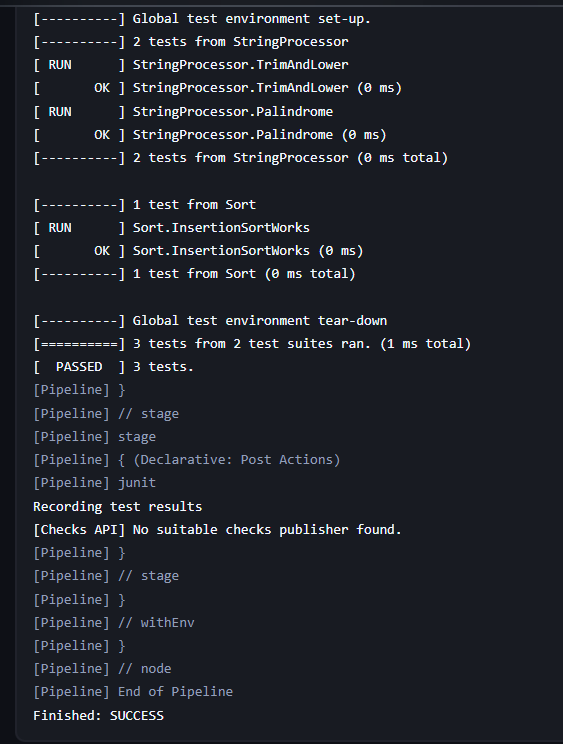
\includegraphics[width=\linewidth]{image2.png}
        \end{subfigure}
        \vfill
        \begin{subfigure}{1.0\textwidth}
            \centering
            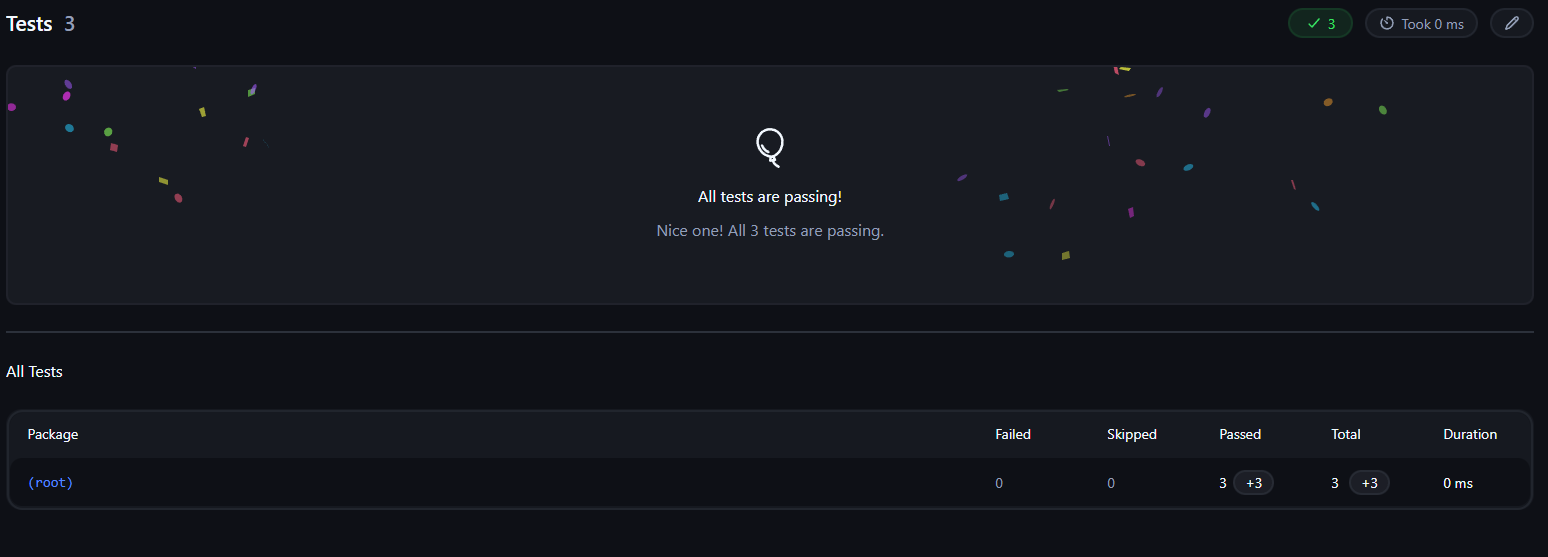
\includegraphics[width=\linewidth]{image3.png}
        \end{subfigure}
    \end{figure}

    \textbf{\underline{Висновок:}}
    У ході виконання лабораторної роботи було розгорнуто систему безперервної інтеграції (Continuous Integration) на основі сервера Jenkins. Було створено віддалений репозиторій у системі керування версіями Gitea та реалізовано повний цикл збірки програмного проєкту з використанням інструментів \texttt{CMake}, \texttt{GoogleTest} і \texttt{MSBuild}.

    У Jenkins було налаштовано Pipeline із трьома основними етапами:
    \begin{itemize}
        \item \textbf{Checkout} — автоматичне отримання коду з віддаленого репозиторію Gitea за допомогою токена доступу (\texttt{credentialsId}).
        \item \textbf{Build} — компіляція проєкту за допомогою \texttt{CMake} та генератора \texttt{Visual Studio 17 2022}.
        \item \textbf{Test} — запуск модульних тестів (\texttt{unit\_tests.exe}) і автоматичне формування звіту у форматі \texttt{JUnit XML}.
    \end{itemize}

    Отриманий файл звіту про тести було успішно імпортовано у Jenkins, що дало змогу переглядати результати виконання тестів безпосередньо через веб-інтерфейс. Також було перевірено працездатність збірки та тестів при підключенні репозиторію через SCM (Pipeline script from SCM).

    Таким чином, у результаті виконання лабораторної роботи:
    \begin{enumerate}
        \item Ознайомлено з принципами роботи системи безперервної інтеграції Jenkins.
        \item Автоматизовано процес збірки, тестування та формування звітів.
        \item Реалізовано практичне підключення до системи контролю версій Gitea з використанням токенів доступу.
    \end{enumerate}

    Робота продемонструвала переваги CI-підходу у забезпеченні стабільності, відтворюваності та контрольованості процесу розробки програмного забезпечення.

  \newpage

  \begin{center}
    \phantomsection\label{sec:concl}%
    \textbf{\Large 5. ВИСНОВКИ}
  \end{center}

  У межах курсової роботи опановано базові інструменти роботи з Unix-подібними системами:
керування версіями у Git (rebase, cherry-pick, squash/drop, форматування патчів), збірку та
автоматизацію за допомогою Make, написання та налагодження bash-скриптів, а також
знайомство з CI/CD на основі Jenkins. Усі етапи супроводжувалися практичними завданнями
(робота з історією комітів, розв’язання конфліктів, перенесення змін між репозиторіями,
додавання нової функціональності), що підтверджує сформовані навички. Отримані результати
дозволяють впевнено застосовувати інструменти командного рядка, системи контролю версій та
засоби безперервної інтеграції для подальшої розробки й підтримки програмних проєктів.

  \newpage

  \begin{center}
    \phantomsection\label{sec:sources}%
    \textbf{\Large 6. СПИСОК ВИКОРИСТАНИХ ДЖЕРЕЛ}
  \end{center}

  \begin{enumerate}
  \item Pro Git: офіційна книга про систему контролю версій Git 
        [Електронний ресурс]. – Режим доступу: 
        \url{https://git-scm.com/book/uk/v2}.

  \item GNU Make: Official Manual [Електронний ресурс]. – Режим доступу: 
        \url{https://www.gnu.org/software/make/manual/make.html}.

  \item Makefile cheatsheet / Devhints [Електронний ресурс]. – Режим доступу: 
        \url{https://devhints.io/makefile}.

  \item GNU Bash Reference Manual [Електронний ресурс]. – Режим доступу: 
        \url{https://www.gnu.org/savannah-checkouts/gnu/bash/manual/bash.html}.

  \item Jenkins User Documentation [Електронний ресурс]. – Режим доступу: 
        \url{https://www.jenkins.io/doc/}.

  \item Жабін В.\,І., Жуков І.\,А., Клименко І.\,А., Ткаченко В.\,В. 
        \textit{Прикладна теорія цифрових автоматів}. – 2-ге вид., доопрацьоване.
\end{enumerate}

\end{document}